\documentclass[12pt, a4paper]{report}

% ── Encoding & Font ────────────────────────────────────────────────────────────
% Tự chọn cấu hình theo engine: pdfLaTeX (T5/inputenc) hoặc XeLaTeX/LuaLaTeX (fontspec)
\usepackage{iftex}
\ifPDFTeX
  \usepackage[utf8]{inputenc}
  \usepackage[T5]{fontenc}
\else
  % XeLaTeX / LuaLaTeX: dùng Unicode + fontspec
  \usepackage{fontspec}
  \defaultfontfeatures{Ligatures=TeX}
  % Latin Modern hỗ trợ đầy đủ ký tự tiếng Việt; đổi font tại đây nếu muốn
  \setmainfont{Latin Modern Roman}
\fi
\usepackage[vietnamese,english]{babel}

% ── Page Layout ───────────────────────────────────────────────────────────────
\usepackage[
  top=3cm, bottom=3cm,
  left=3.5cm, right=2cm
]{geometry}
\usepackage{setspace}
\onehalfspacing

% ── Math ──────────────────────────────────────────────────────────────────────
\usepackage{amsmath, amssymb, amsthm}
\usepackage{bm}

% ── Graphics & Tables ─────────────────────────────────────────────────────────
\usepackage{graphicx}
\graphicspath{{figures/}}
\usepackage{float}
\usepackage{booktabs}
\usepackage{multirow}
\usepackage{array}
\usepackage{longtable}
\usepackage[table,xcdraw]{xcolor}
\usepackage{enumitem}

% ── Diagrams (TikZ) ───────────────────────────────────────────────────────────
\usepackage{tikz}
\usetikzlibrary{arrows.meta, positioning, shapes.geometric, fit, backgrounds}

% ── Code Listings ─────────────────────────────────────────────────────────────
\usepackage{listings}
\lstset{
  basicstyle=\ttfamily\small,
  breaklines=true,
  frame=single,
  numbers=left,
  numberstyle=\tiny,
  keywordstyle=\color{blue},
  commentstyle=\color{gray},
  showstringspaces=false,
  columns=fullflexible,
  keepspaces=true,
  extendedchars=true,
  upquote=true,
}

% ── Hyperlinks ────────────────────────────────────────────────────────────────
\usepackage[
  colorlinks=true,
  linkcolor=black,
  citecolor=blue,
  urlcolor=blue
]{hyperref}

% ── Caption ───────────────────────────────────────────────────────────────────
\usepackage{caption}
\usepackage{subcaption}

% ── Bibliography ──────────────────────────────────────────────────────────────
\usepackage[backend=biber, style=ieee, sorting=none]{biblatex}
\addbibresource{references.bib}

% ── Theorem environments ──────────────────────────────────────────────────────
\newtheorem{definition}{Định nghĩa}[chapter]
\newtheorem{theorem}{Định lý}[chapter]

% ── Custom commands ───────────────────────────────────────────────────────────
\newcommand{\auc}{\text{ROC-AUC}}
\newcommand{\prauc}{\text{PR-AUC}}
\newcommand{\system}{\textit{InternHub}}

% Chèn ảnh an toàn: nếu file chưa có thì hiện khung placeholder, KHÔNG lỗi compile.
\newcommand{\safefig}[2]{%
  \IfFileExists{figures/#1}%
    {\includegraphics[width=#2]{#1}}%
    {\fbox{\parbox[c][4cm][c]{#2}{\centering\itshape [Chèn hình \texttt{#1} vào thư mục \texttt{figures/}]}}}%
}

% ──────────────────────────────────────────────────────────────────────────────
\begin{document}

% ── Title page ────────────────────────────────────────────────────────────────
\begin{titlepage}
  \centering
  \IfFileExists{figures/uit_logo.png}{\includegraphics[width=3cm]{uit_logo.png}\\[0.5cm]}{}
  {\large \textbf{ĐẠI HỌC QUỐC GIA TP. HỒ CHÍ MINH}}\\
  {\large \textbf{TRƯỜNG ĐẠI HỌC CÔNG NGHỆ THÔNG TIN}}\\[2cm]

  {\LARGE \textbf{HỆ THỐNG PHÂN LOẠI VÀ GỢI Ý}}\\[0.3cm]
  {\LARGE \textbf{PHỎNG VẤN IT DỰA TRÊN KNOWLEDGE TRACING}}\\[0.3cm]
  {\large \textbf{(InternHub KT Recommendation System)}}\\[2cm]

  {\large \textbf{Nhóm sinh viên thực hiện}}\\[0.4cm]
  \begin{tabular}{lll}
    Mai Dương Hải Đăng & 24520253 & 24520253@gm.uit.edu.vn \\
    Tạ Gia Khiêm       & 24520805 & 24520805@gm.uit.edu.vn \\
    Nguyễn Sỹ Huỳnh    & 24520716 & 24520716@gm.uit.edu.vn \\
    Nguyễn Ngọc Nam    & 24521114 & 24521114@gm.uit.edu.vn \\
  \end{tabular}\\[1cm]

  \begin{tabular}{ll}
    \textbf{Giáo viên hướng dẫn:} & TS. Nguyễn Văn Kiệt \\
  \end{tabular}\\[2cm]

  {\large TP. Hồ Chí Minh, 2026}
\end{titlepage}

% ── Front matter ──────────────────────────────────────────────────────────────
\pagenumbering{roman}

\chapter*{Lời Cam Đoan}
\addcontentsline{toc}{chapter}{Lời Cam Đoan}

Tôi xin cam đoan khóa luận \textit{``Hệ thống phân loại và gợi ý phỏng vấn IT dựa trên Knowledge Tracing (InternHub)''} là công trình nghiên cứu của riêng tôi dưới sự hướng dẫn của giáo viên hướng dẫn. Các kết quả, số liệu thực nghiệm trình bày trong khóa luận là trung thực và được tạo ra từ chính pipeline dữ liệu, mã nguồn và các thí nghiệm do tôi thực hiện.

Toàn bộ question bank được xây dựng từ các nguồn câu hỏi phỏng vấn công khai (kèm trích dẫn) kết hợp sinh tự động bằng mô hình ngôn ngữ lớn; dữ liệu huấn luyện Knowledge Tracing là dữ liệu \textbf{mô phỏng tổng hợp}, không sử dụng dữ liệu cá nhân của người dùng thật. Mọi tài liệu tham khảo đều được trích dẫn đầy đủ trong danh mục Tài liệu tham khảo.

Tôi xin chịu hoàn toàn trách nhiệm về tính trung thực của khóa luận.

\vspace{1.5cm}
\hfill\begin{tabular}{c}
TP. Hồ Chí Minh, 2026 \\
Nhóm sinh viên thực hiện \\[2.5cm]
Mai Dương Hải Đăng \quad Tạ Gia Khiêm \\
Nguyễn Sỹ Huỳnh \quad Nguyễn Ngọc Nam \\
\end{tabular}

\chapter*{Lời Cảm Ơn}
\addcontentsline{toc}{chapter}{Lời Cảm Ơn}

Tôi xin gửi lời cảm ơn chân thành đến giáo viên hướng dẫn đã định hướng đề tài, góp ý về phương pháp luận và đồng hành trong suốt quá trình thực hiện khóa luận. Tôi cũng xin cảm ơn quý thầy cô Trường Đại học Công nghệ Thông tin -- ĐHQG TP.HCM đã trang bị nền tảng kiến thức về Học máy, Khai phá dữ liệu và Kỹ thuật phần mềm, làm cơ sở cho công trình này.

Cuối cùng, tôi xin cảm ơn gia đình và bạn bè đã luôn động viên, hỗ trợ trong thời gian thực hiện đề tài.

\vspace{0.5cm}
\hfill\textit{Tác giả khóa luận}

\chapter*{Tóm Tắt}
\addcontentsline{toc}{chapter}{Tóm Tắt}

Khóa luận đề xuất và xây dựng \system{} -- một hệ thống luyện phỏng vấn IT cá nhân hóa tích hợp \textbf{Knowledge Tracing (KT)} cho ba vai trò dữ liệu phổ biến: Data Analyst (DA), Data Scientist (DS) và Data Engineer (DE). Hệ thống giải quyết hai hạn chế của các nền tảng luyện phỏng vấn hiện nay: thiếu cá nhân hóa theo năng lực và không theo dõi được quỹ đạo kiến thức của người học.

Về dữ liệu, khóa luận xây dựng question bank đa dạng (5 loại câu hỏi, 17 Knowledge Components) bằng pipeline kết hợp thu thập từ các nguồn công khai và sinh tự động bằng LLM kèm kiểm định chất lượng; đồng thời thiết kế pipeline mô phỏng tương tác dựa trên Item Response Theory (IRT) để tạo bộ dữ liệu huấn luyện KT (1.000 người dùng ảo, $\sim$40.000 tương tác). Về mô hình, khóa luận huấn luyện và so sánh ba họ KT -- BKT, DKT, SAKT -- cùng biến thể \textit{quality label} liên tục. Kết quả trên tập kiểm tra cho thấy mọi mô hình KT vượt baseline (ROC-AUC $\approx$ 0.68 so với 0.50); biến thể \textbf{DKT-Quality} đạt PR-AUC và RMSE tốt nhất trong nhóm neural.

Về hệ thống, khóa luận thiết kế cơ chế cập nhật năng lực thời gian thực bằng cách kết hợp dự đoán KT (70\%) và trung bình trượt mũ EMA (30\%), tích hợp vào engine gợi ý theo chiến lược \textit{zone of proximal development} và bài kiểm tra thích nghi hai giai đoạn (Multi-Stage Testing). Toàn bộ được hiện thực thành ứng dụng web hoàn chỉnh (React + FastAPI + Streamlit) với chấm điểm tự động bằng Gemini LLM và cơ chế chấm dự phòng cục bộ.

\textbf{Từ khóa:} Knowledge Tracing, Deep Knowledge Tracing, Item Response Theory, Hệ thống gợi ý, Computerized Adaptive Testing, Luyện phỏng vấn IT.

\vspace{0.6cm}
\begin{center}\rule{0.5\textwidth}{0.4pt}\end{center}
\vspace{0.3cm}

\noindent\textbf{\large Abstract}

\smallskip
This thesis proposes and implements \system{}, a personalized IT interview-practice platform powered by \textbf{Knowledge Tracing (KT)} for three popular data roles: Data Analyst, Data Scientist, and Data Engineer. It addresses two limitations of existing platforms: the lack of competency-based personalization and the inability to track a learner's knowledge trajectory. A diverse question bank (5 question types, 17 Knowledge Components) is built through a hybrid pipeline of public-source collection and LLM generation with quality control, while an IRT-based simulation pipeline produces the KT training data (1{,}000 virtual users, $\sim$40{,}000 interactions). Three KT model families -- BKT, DKT, SAKT -- are trained and compared, including a continuous \textit{quality-label} variant; all KT models beat the baseline (ROC-AUC $\approx$ 0.68 vs.\ 0.50), with DKT-Quality achieving the best PR-AUC and RMSE among neural models. A real-time skill-update mechanism blends KT prediction (70\%) with an exponential moving average (30\%), feeding a zone-of-proximal-development recommender and a two-stage adaptive test. The whole pipeline is realized as a complete web application (React + FastAPI + Streamlit) with automatic LLM-based grading and a local fallback grader.

\noindent\textbf{Keywords:} Knowledge Tracing, Deep Knowledge Tracing, Item Response Theory, Recommendation System, Computerized Adaptive Testing, IT Interview Preparation.


\tableofcontents
\listoffigures
\listoftables

\chapter*{Danh Mục Từ Viết Tắt}
\addcontentsline{toc}{chapter}{Danh Mục Từ Viết Tắt}

\begin{longtable}{ll}
\toprule
\textbf{Từ viết tắt} & \textbf{Diễn giải} \\
\midrule
\endfirsthead
\toprule
\textbf{Từ viết tắt} & \textbf{Diễn giải} \\
\midrule
\endhead
\bottomrule
\endfoot
KT     & Knowledge Tracing -- Theo dõi tri thức \\
BKT    & Bayesian Knowledge Tracing \\
DKT    & Deep Knowledge Tracing \\
SAKT   & Self-Attentive Knowledge Tracing \\
IRT    & Item Response Theory -- Lý thuyết ứng đáp câu hỏi \\
CAT    & Computerized Adaptive Testing -- Kiểm tra thích nghi \\
MST    & Multi-Stage Testing -- Kiểm tra nhiều giai đoạn \\
KC     & Knowledge Component -- Thành phần tri thức \\
EMA    & Exponential Moving Average -- Trung bình trượt mũ \\
ZPD    & Zone of Proximal Development -- Vùng phát triển gần \\
LLM    & Large Language Model -- Mô hình ngôn ngữ lớn \\
ROC-AUC & Area Under the ROC Curve \\
PR-AUC & Area Under the Precision-Recall Curve \\
RMSE   & Root Mean Squared Error \\
LSTM   & Long Short-Term Memory \\
SPA    & Single-Page Application \\
API    & Application Programming Interface \\
EDA    & Exploratory Data Analysis -- Phân tích khám phá dữ liệu \\
QC     & Quality Control -- Kiểm định chất lượng \\
DA / DS / DE & Data Analyst / Data Scientist / Data Engineer \\
\end{longtable}

\noindent\textbf{17 Knowledge Components (KC) theo vai trò:}

\begin{longtable}{lll}
\toprule
\textbf{Vai trò} & \textbf{Mã KC} & \textbf{Ý nghĩa} \\
\midrule
\endfirsthead
\toprule
\textbf{Vai trò} & \textbf{Mã KC} & \textbf{Ý nghĩa} \\
\midrule
\endhead
\bottomrule
\endfoot
\multirow{5}{*}{DA}
 & SQL\_DATABASE               & SQL \& cơ sở dữ liệu \\
 & BI\_VISUALIZATION           & Trực quan hóa \& BI \\
 & STATISTICS\_EXPERIMENTATION & Thống kê \& thực nghiệm \\
 & ANALYTICS\_BUSINESS         & Phân tích nghiệp vụ \\
 & PYTHON\_ANALYTICS           & Python cho phân tích \\
\midrule
\multirow{7}{*}{DS}
 & ALGORITHM\_THEORY           & Thuật toán \& lý thuyết ML \\
 & EVALUATION\_METRICS         & Độ đo đánh giá mô hình \\
 & DATA\_PREPROCESSING         & Tiền xử lý dữ liệu \\
 & DEEP\_LEARNING              & Học sâu \\
 & NLP                         & Xử lý ngôn ngữ tự nhiên \\
 & TIME\_SERIES                & Chuỗi thời gian \\
 & MLOPS                       & Vận hành ML (MLOps) \\
\midrule
\multirow{5}{*}{DE}
 & DATA\_PIPELINE              & Đường ống dữ liệu (ETL/ELT) \\
 & DATA\_ARCHITECTURE\_MODELING & Kiến trúc \& mô hình hóa dữ liệu \\
 & BIG\_DATA\_CLOUD\_TOOLS      & Big data \& công cụ cloud \\
 & DATABASE\_INTERNALS         & Cơ chế nội tại CSDL \\
 & SYSTEM\_ARCHITECTURE        & Kiến trúc hệ thống \\
\end{longtable}


% ── Main matter ───────────────────────────────────────────────────────────────
\pagenumbering{arabic}
\setcounter{page}{1}

\chapter{Giới Thiệu}
\label{chap:intro}

% ─────────────────────────────────────────────────────────────────────────────
\section{Đặt Vấn Đề}
\label{sec:motivation}

Thị trường tuyển dụng nhân lực công nghệ thông tin tại Việt Nam và trên thế giới đang chứng kiến sự cạnh tranh ngày càng gay gắt. Theo khảo sát của TopDev (2024) \cite{topdev2024}, hơn 70\% ứng viên IT tại Việt Nam thừa nhận chưa chuẩn bị đủ kỹ năng kỹ thuật cần thiết trước các vòng phỏng vấn, trong khi phần lớn các nền tảng luyện phỏng vấn hiện có (LeetCode, HackerRank, Pramp) chủ yếu tập trung vào lập trình thuật toán, thiếu nội dung dành riêng cho ba vai trò dữ liệu phổ biến nhất: Data Analyst (DA), Data Scientist (DS) và Data Engineer (DE).

Hai thách thức cốt lõi tồn tại với các nền tảng luyện phỏng vấn hiện tại:

\textbf{(1) Thiếu cá nhân hóa theo năng lực.} Hầu hết hệ thống cung cấp câu hỏi theo cách tĩnh (static), không phản ánh được trình độ thực tế của từng ứng viên. Người dùng có kinh nghiệm phải làm lại các câu hỏi quá dễ, trong khi người mới bắt đầu có thể nản lòng với câu hỏi ngoài tầm. Vấn đề này tương ứng với khái niệm \textit{zone of proximal development} trong tâm lý học giáo dục \cite{vygotsky1978mind} -- câu hỏi hiệu quả nhất là câu hỏi hơi khó hơn năng lực hiện tại của người học một chút.

\textbf{(2) Không theo dõi được quỹ đạo kiến thức.} Hệ thống hiện có không duy trì và cập nhật trạng thái kiến thức (knowledge state) của người học theo thời gian. Do đó, sau mỗi phiên luyện tập, hệ thống không biết người dùng đã tiến bộ ở điểm nào, còn yếu ở kỹ năng nào, và câu hỏi tiếp theo nên theo hướng nào.

Knowledge Tracing (KT) \cite{corbett1994knowledge} là hướng giải quyết được nghiên cứu nhiều trong lĩnh vực Educational Data Mining, giúp mô hình hóa và dự đoán trạng thái kiến thức của người học qua lịch sử tương tác. Các mô hình KT từ Bayesian Knowledge Tracing \cite{corbett1994knowledge} đến Deep Knowledge Tracing \cite{piech2015deep} và Self-Attentive Knowledge Tracing \cite{pandey2019self} đã chứng minh hiệu quả trong môi trường học thuật (MOOC, bài tập toán, ngôn ngữ). Tuy nhiên, việc áp dụng KT cho bài toán luyện phỏng vấn IT -- với đặc thù câu hỏi mở, chấm điểm tự động bằng LLM và nhiều loại câu hỏi (lý thuyết, coding, tình huống) -- vẫn là một bài toán mở.

Luận văn này đề xuất và xây dựng \system{}, một hệ thống luyện phỏng vấn IT tích hợp KT, nhằm giải quyết đồng thời hai thách thức trên: theo dõi năng lực tự động và gợi ý câu hỏi cá nhân hóa theo từng vai trò nghề nghiệp.

% ─────────────────────────────────────────────────────────────────────────────
\section{Mục Tiêu Nghiên Cứu}
\label{sec:objectives}

Luận văn đặt ra bốn mục tiêu chính:

\begin{enumerate}
  \item \textbf{Xây dựng bộ dữ liệu luyện KT phù hợp cho bài toán phỏng vấn IT.} Do thiếu dữ liệu thực, luận văn thiết kế pipeline mô phỏng dữ liệu tổng hợp có tính chất thực tế cao, kết hợp IRT \cite{embretson2000item} để sinh hành vi người dùng và LLM để xây dựng question bank đa dạng cho ba vai trò DA/DS/DE.

  \item \textbf{Huấn luyện và so sánh các mô hình KT.} Triển khai và đánh giá ba họ mô hình -- BKT \cite{corbett1994knowledge}, DKT \cite{piech2015deep}, SAKT \cite{pandey2019self} -- với các biến thể sử dụng nhãn nhị phân và quality label liên tục. Phân tích điểm mạnh/yếu của từng mô hình trên tập dữ liệu phỏng vấn IT.

  \item \textbf{Xây dựng engine gợi ý dựa trên KT.} Thiết kế cơ chế cập nhật skill vector bằng cách kết hợp KT prediction (70\%) và EMA (30\%), tích hợp vào pipeline đề xuất câu hỏi theo chiến lược zone of proximal development, có hỗ trợ Computerized Adaptive Testing (CAT) hai giai đoạn \cite{wainer2000computerized}.

  \item \textbf{Tích hợp vào ứng dụng web hoàn chỉnh.} Xây dựng \system{} -- giao diện React SPA được phục vụ qua Streamlit, kết nối với FastAPI backend -- hỗ trợ chấm điểm tự động bằng Gemini LLM và fallback local rubric \cite{team2023gemini}.
\end{enumerate}

% ─────────────────────────────────────────────────────────────────────────────
\section{Phạm Vi Nghiên Cứu}
\label{sec:scope}

\textbf{Trong phạm vi:}
\begin{itemize}
  \item Ba vai trò nghề nghiệp: Data Analyst (DA), Data Scientist (DS), Data Engineer (DE).
  \item 17 Knowledge Components (KC) phân bổ theo vai trò: DA (5 KC), DS (7 KC), DE (5 KC).
  \item Bộ câu hỏi gồm 5 loại: trắc nghiệm (MC\_SINGLE), đúng/sai (TRUE\_FALSE), điền chỗ trống (FILL\_BLANK), lý thuyết mở (THEORY), và coding (CODING/CODING\_EXERCISE).
  \item Dữ liệu training KT: 1{,}000 người dùng mô phỏng, $\sim$40{,}000 tương tác.
  \item Chấm điểm câu hỏi mở bằng Gemini 3.5 Flash với local rubric fallback.
\end{itemize}

\textbf{Ngoài phạm vi:}
\begin{itemize}
  \item Thu thập và sử dụng dữ liệu người dùng thực (do giới hạn thời gian và quyền riêng tư).
  \item Triển khai production với load balancing và autoscaling.
  \item Đánh giá A/B testing so với các hệ thống thương mại.
  \item Hỗ trợ các ngôn ngữ lập trình thực thi trong sandbox (chỉ hiển thị).
\end{itemize}

% ─────────────────────────────────────────────────────────────────────────────
\section{Đóng Góp Chính}
\label{sec:contributions}

Luận văn có bốn đóng góp chính:

\begin{enumerate}
  \item \textbf{Pipeline xây dựng dữ liệu phỏng vấn IT tổng hợp}: Một pipeline đầy đủ từ sinh câu hỏi (LLM), tạo người dùng ảo (correlated Gaussian skill), đến mô phỏng tương tác (IRT + power-based graded response). Pipeline này có thể tái sử dụng cho các bài toán KT trong lĩnh vực nghề nghiệp khác.

  \item \textbf{So sánh hệ thống KT với quality label}: Đề xuất và đánh giá biến thể DKT-Quality sử dụng điểm chất lượng liên tục $\in \{0, 0.5, 1\}$ thay vì nhãn nhị phân, cho thấy cải thiện đáng kể về RMSE và PR-AUC trên bộ dữ liệu phỏng vấn IT.

  \item \textbf{Cơ chế tích hợp KT--EMA cho real-time skill update}: Công thức blend KT(70\%) + EMA(30\%) với ngưỡng kích hoạt tối thiểu 3 tương tác, giải quyết bài toán cold-start và đảm bảo tính ổn định trong giai đoạn đầu.

  \item \textbf{Hệ thống luyện phỏng vấn IT end-to-end}: Ứng dụng \system{} hoàn chỉnh tích hợp KT, 2-Stage Branching CAT, chấm điểm LLM, và giao diện React với FastAPI backend -- tất cả trong một codebase duy nhất có thể chạy local.
\end{enumerate}

% ─────────────────────────────────────────────────────────────────────────────
\section{Cấu Trúc Luận Văn}
\label{sec:structure}

Phần còn lại của luận văn được tổ chức như sau:

\textbf{Chương \ref{chap:theory} -- Cơ Sở Lý Thuyết:} Trình bày nền tảng lý thuyết của Knowledge Tracing (BKT, DKT, SAKT), Item Response Theory, và hệ thống gợi ý trong ngữ cảnh luyện phỏng vấn. Đồng thời khảo sát các công trình liên quan trong lĩnh vực.

\textbf{Chương \ref{chap:data} -- Xây Dựng Dữ Liệu và Phân Tích Khám Phá:} Mô tả chi tiết pipeline xây dựng question bank và dữ liệu mô phỏng, kết hợp với phân tích EDA toàn diện về đặc tính bộ dữ liệu.

\textbf{Chương \ref{chap:experiment} -- Thực Nghiệm và Đánh Giá:} Trình bày thiết kế thực nghiệm, kết quả huấn luyện và đánh giá các mô hình KT, phân tích so sánh, và thảo luận về hạn chế.

\textbf{Chương \ref{chap:conclusion} -- Kết Luận và Hướng Phát Triển:} Tổng kết kết quả đạt được, đóng góp, và đề xuất hướng phát triển cho nghiên cứu tương lai.

\chapter{Cơ Sở Lý Thuyết}
\label{chap:theory}

\section{Knowledge Tracing}
\label{sec:kt}

Knowledge Tracing (KT) là bài toán theo dõi và dự đoán trạng thái kiến thức của người học qua thời gian, dựa trên lịch sử tương tác với các bài tập. Cho một chuỗi tương tác $\{(q_1, r_1), (q_2, r_2), \ldots, (q_t, r_t)\}$ trong đó $q_t$ là câu hỏi tại thời điểm $t$ và $r_t \in \{0, 1\}$ là kết quả (đúng/sai), mục tiêu của KT là dự đoán xác suất trả lời đúng câu hỏi tiếp theo $q_{t+1}$:
\begin{equation}
  p(r_{t+1} = 1 \mid q_{t+1}, q_1, r_1, \ldots, q_t, r_t)
\end{equation}

Trong hệ thống \system{}, bài toán KT được áp dụng để theo dõi năng lực của ứng viên trên 17 nhóm kỹ năng (Knowledge Components -- KC) thuộc ba vai trò nghề nghiệp IT: Data Analyst (DA), Data Scientist (DS) và Data Engineer (DE).

\subsection{Bayesian Knowledge Tracing (BKT)}
\label{subsec:bkt}

BKT \cite{corbett1994knowledge} mô hình hóa từng KC như một chuỗi Markov ẩn (Hidden Markov Model -- HMM) với hai trạng thái: \textit{chưa thành thạo} ($L=0$) và \textit{thành thạo} ($L=1$). Mô hình được đặc trưng bởi bốn tham số cho mỗi KC:

\begin{itemize}
  \item $P(L_0)$: xác suất ban đầu người học đã thành thạo KC.
  \item $P(T)$: xác suất chuyển từ chưa thành thạo sang thành thạo sau mỗi lần thực hành.
  \item $P(S)$: xác suất trả lời sai dù đã thành thạo (\textit{slip}).
  \item $P(G)$: xác suất trả lời đúng dù chưa thành thạo (\textit{guess}).
\end{itemize}

Xác suất trả lời đúng tại bước $t$ được tính:
\begin{equation}
  P(r_t = 1) = P(L_t)(1 - P(S)) + (1 - P(L_t))P(G)
\end{equation}

Sau mỗi quan sát, trạng thái thành thạo được cập nhật theo Bayes:
\begin{equation}
  P(L_t \mid r_t = 1) = \frac{P(L_t)(1 - P(S))}{P(r_t = 1)}
\end{equation}

\begin{equation}
  P(L_{t+1}) = P(L_t \mid r_t) + (1 - P(L_t \mid r_t)) \cdot P(T)
\end{equation}

Tham số của BKT được ước lượng bằng thuật toán Expectation-Maximization (EM) hoặc tối ưu hóa trực tiếp L-BFGS-B trên log-likelihood. Ưu điểm của BKT là khả năng diễn giải cao và hiệu quả trên dữ liệu nhỏ; hạn chế là giả định độc lập giữa các KC và không mô hình hóa được tương tác bài tập phức tạp.

\subsection{Deep Knowledge Tracing (DKT)}
\label{subsec:dkt}

DKT \cite{piech2015deep} thay thế mô hình xác suất của BKT bằng mạng nơ-ron hồi quy (LSTM), cho phép học được biểu diễn ẩn phong phú hơn cho trạng thái kiến thức của người học. Đầu vào tại mỗi bước $t$ là vector one-hot mã hóa cặp $(q_t, r_t)$, có chiều $2 \cdot |\mathcal{Q}|$ với $|\mathcal{Q}|$ là số lượng câu hỏi (hoặc KC).

\begin{equation}
  \mathbf{h}_t = \text{LSTM}(\mathbf{x}_t, \mathbf{h}_{t-1})
\end{equation}
\begin{equation}
  \hat{y}_{t+1} = \sigma(\mathbf{W} \cdot \mathbf{h}_t + \mathbf{b})
\end{equation}

trong đó $\hat{y}_{t+1}$ là xác suất trả lời đúng câu hỏi tiếp theo, $\sigma$ là hàm sigmoid.

Trong \system{}, DKT được mở rộng với \textbf{quality label}: thay vì nhãn nhị phân $r_t \in \{0,1\}$, mô hình sử dụng điểm chất lượng liên tục $r_t \in [0, 1]$ phản ánh mức độ thành thạo (điểm tự đánh giá sau phỏng vấn). Hàm mất mát chuyển từ Binary Cross-Entropy sang Mean Squared Error:
\begin{equation}
  \mathcal{L}_{\text{quality}} = \frac{1}{T} \sum_{t=1}^{T} (r_t - \hat{y}_t)^2
\end{equation}

\subsection{Self-Attentive Knowledge Tracing (SAKT)}
\label{subsec:sakt}

SAKT \cite{pandey2019self} thay thế kiến trúc hồi quy của DKT bằng cơ chế self-attention, cho phép mô hình học được mối liên hệ trực tiếp giữa các KC liên quan trong lịch sử tương tác.

Cho chuỗi tương tác $\{(q_1, r_1), \ldots, (q_{t-1}, r_{t-1})\}$, SAKT xây dựng:
\begin{itemize}
  \item \textbf{Exercise embedding}: $\mathbf{e}_{q_t} \in \mathbb{R}^d$ cho câu hỏi cần dự đoán.
  \item \textbf{Interaction embedding}: $\mathbf{m}_s = \mathbf{e}_{q_s} + \mathbf{r}_s$ cho mỗi bước lịch sử.
\end{itemize}

Attention score giữa câu hỏi $q_t$ và bước lịch sử $s$ được tính:
\begin{equation}
  a_{t,s} = \frac{(\mathbf{e}_{q_t} \mathbf{W}^Q)(\mathbf{m}_s \mathbf{W}^K)^\top}{\sqrt{d}}
\end{equation}

\begin{equation}
  \hat{y}_t = \sigma\left(\mathbf{W}_o \cdot \sum_s \text{softmax}(a_{t,s}) \cdot \mathbf{m}_s \mathbf{W}^V\right)
\end{equation}

Ưu điểm của SAKT là khả năng song song hóa (không sequential như LSTM) và diễn giải được attention weight để hiểu KC nào ảnh hưởng đến dự đoán.

\section{Item Response Theory (IRT)}
\label{sec:irt}

Item Response Theory \cite{embretson2000item} là khung lý thuyết mô hình hóa mối quan hệ giữa năng lực người học $\theta$ và xác suất trả lời đúng câu hỏi $i$. Mô hình 3PL (3-Parameter Logistic) được dùng trong simulation:

\begin{equation}
  P(r = 1 \mid \theta, a_i, b_i, c_i) = c_i + (1 - c_i) \cdot \frac{1}{1 + e^{-a_i(\theta - b_i)}}
\end{equation}

trong đó $a_i$ là độ phân biệt (discrimination), $b_i$ là độ khó (difficulty), $c_i$ là xác suất đoán ngẫu nhiên (guessing). Trong \system{}, tham số IRT được ánh xạ từ cấu hình độ khó EASY/MEDIUM/HARD với $b \in \{0.30, 0.55, 0.80\}$.

\section{Recommendation System cho Interview Practice}
\label{sec:recsys}

Hệ thống gợi ý trong \system{} kết hợp KT và Collaborative Filtering để đề xuất câu hỏi phù hợp với trình độ hiện tại của ứng viên. Cụ thể, sau mỗi phiên luyện tập, vector năng lực $\bm{\theta}_u \in \mathbb{R}^{17}$ của người dùng $u$ (17 KC) được cập nhật bởi KT model, sau đó được dùng để xếp hạng câu hỏi theo chiến lược \textit{zone of proximal development}: ưu tiên câu hỏi thuộc KC yếu và độ khó phù hợp.

\section{Cập Nhật Năng Lực Thời Gian Thực: EMA và Blend KT--EMA}
\label{sec:ema}

Mô hình KT cho dự đoán tốt khi đã có đủ lịch sử tương tác, nhưng kém ổn định ở giai đoạn đầu (\textit{cold-start}) khi người dùng mới chỉ trả lời vài câu. Để giải quyết, \system{} kết hợp KT với \textbf{Exponential Moving Average (EMA)} -- một bộ ước lượng trực tuyến đơn giản, ổn định và không cần lịch sử dài.

Với mỗi KC, sau khi quan sát điểm số $s_t \in [0,1]$ tại bước $t$, giá trị EMA được cập nhật:
\begin{equation}
  \theta^{\text{EMA}}_t = \alpha \, s_t + (1 - \alpha)\,\theta^{\text{EMA}}_{t-1},
  \qquad \alpha = 0.35 .
\end{equation}

EMA luôn chạy ngay từ tương tác đầu tiên, cung cấp ước lượng năng lực thô. Khi lịch sử đạt tối thiểu $H_{\min} = 3$ tương tác, dự đoán KT được kích hoạt và \textbf{blend} với EMA theo trọng số cố định:
\begin{equation}
  \hat{\theta}_t = \lambda \, \theta^{\text{KT}}_t + (1 - \lambda)\,\theta^{\text{EMA}}_t,
  \qquad \lambda = 0.70 .
  \label{eq:blend}
\end{equation}

Công thức~\eqref{eq:blend} là một trong các đóng góp chính của khóa luận. Lựa chọn $\lambda = 0.7$ cho KT trọng số trội (vì KT nắm bắt được động lực chuỗi và quan hệ giữa các KC), trong khi giữ $0.3$ cho EMA nhằm \textit{ổn định hóa} dự đoán, chống dao động mạnh khi KT gặp chuỗi nhiễu. Ngưỡng $H_{\min}=3$ đảm bảo KT chỉ tham gia khi đã có đủ ngữ cảnh, còn trước đó hệ thống dùng EMA thuần. Hằng số $\lambda$ và $H_{\min}$ được giữ \textbf{nhất quán} giữa backend Python và frontend để bảo đảm con số hiển thị đồng bộ trên toàn hệ thống (xem Chương~\ref{chap:system}).

\section{Các Công Trình Liên Quan}
\label{sec:related}

\textbf{Knowledge Tracing.} Từ BKT \cite{corbett1994knowledge}, các mô hình KT đã phát triển qua DKT \cite{piech2015deep}, DKVMN \cite{zhang2017dynamic}, AKT \cite{ghosh2020context}, và gần đây là các mô hình Transformer-based như SAINT \cite{choi2020towards}. SAKT \cite{pandey2019self} là mô hình attention đầu tiên đơn giản và hiệu quả trong bài toán này.

\textbf{Adaptive Learning Systems.} Knewton \cite{ferreira2017knewton} và các hệ thống ITS (Intelligent Tutoring System) như ASSISTments \cite{heffernan2014assistments} sử dụng KT để cá nhân hóa lộ trình học. Tuy nhiên, các hệ thống này tập trung vào môi trường học thuật, chưa có ứng dụng cụ thể cho phỏng vấn IT.

\textbf{Interview Preparation Systems.} Các nền tảng như LeetCode, HackerRank cung cấp bài tập lập trình nhưng thiếu cơ chế theo dõi kiến thức có cấu trúc. \system{} khác biệt ở chỗ tích hợp KT với question bank đa dạng (lý thuyết, thực hành, coding) cho ba vai trò DA/DS/DE, đồng thời sử dụng LLM để chấm điểm tự động.

\chapter{Xây Dựng Dữ Liệu và Phân Tích Khám Phá}
\label{chap:data}

Chương này mô tả toàn bộ pipeline xây dựng dữ liệu mô phỏng và phân tích khám phá (EDA) nhằm hiểu rõ đặc tính của bộ dữ liệu trước khi huấn luyện mô hình Knowledge Tracing.

% ─────────────────────────────────────────────────────────────────────────────
\section{Tổng Quan Quy Trình Notebooks}
\label{sec:notebook_pipeline}

Toàn bộ phần huấn luyện Knowledge Tracing được tổ chức thành \textbf{bốn notebook chạy tuần tự}, mỗi notebook nhận trực tiếp đầu ra của notebook trước (Hình~\ref{fig:notebook_pipeline}). Quy trình này tách rõ bốn giai đoạn: khám phá dữ liệu, kỹ thuật đặc trưng, huấn luyện và đánh giá; nhờ đó có thể tái lập từng bước một cách độc lập. Toàn bộ pipeline cố định \texttt{seed = 42}; hai notebook huấn luyện và đánh giá (\texttt{03}, \texttt{04}) chạy trên Kaggle với GPU NVIDIA Tesla T4 và PyTorch 2.6.

\begin{figure}[H]
  \centering
  \begin{tikzpicture}[
    node distance=0.7cm and 0.9cm,
    nb/.style={rectangle, rounded corners, draw, thick, fill=blue!8,
      text width=3.1cm, minimum height=1.25cm, align=center, font=\small},
    io/.style={rectangle, draw, fill=gray!10, text width=3.0cm,
      minimum height=0.9cm, align=center, font=\scriptsize\ttfamily},
    arr/.style={-{Stealth[length=2.2mm]}, thick}
  ]
    \node[io] (raw) {data/raw/*};
    \node[nb, below=of raw] (n1) {\textbf{01\_eda}\\Phân tích khám phá, phát hiện \& fix issue};
    \node[nb, below=of n1] (n2) {\textbf{02\_feature\_engineering}\\Tạo nhãn, encode, build sequences};
    \node[nb, below=of n2] (n3) {\textbf{03\_train\_models}\\Ablation 8 cấu hình KT};
    \node[nb, below=of n3] (n4) {\textbf{04\_evaluation}\\Phân tích sâu, chọn mô hình};

    \node[io, right=of n2] (proc) {data/processed/ *.pkl};
    \node[io, right=of n3] (mdl) {results/models/ metrics/ ablation/};
    \node[io, right=of n4] (plt) {results/plots/*};

    \draw[arr] (raw) -- (n1);
    \draw[arr] (n1) -- (n2);
    \draw[arr] (n2) -- (n3);
    \draw[arr] (n3) -- (n4);
    \draw[arr] (n2) -- (proc);
    \draw[arr] (n3) -- (mdl);
    \draw[arr] (n4) -- (plt);
  \end{tikzpicture}
  \caption{Pipeline bốn notebook chạy tuần tự, từ dữ liệu thô đến mô hình KT triển khai.}
  \label{fig:notebook_pipeline}
\end{figure}

Vai trò tóm tắt của từng notebook như sau:

\begin{itemize}
  \item \textbf{\texttt{01\_eda}} --- Kiểm tra chất lượng dữ liệu thô (null, mất cân bằng, bất thường) và phát hiện các vấn đề cần sửa \emph{trước khi} feature engineering: chuẩn hóa quality thành nhãn nhị phân (cho AUC) và nhãn float (cho RMSE), cảnh báo độ dài chuỗi đồng đều (uniform), và đối chiếu tự đánh giá với năng lực thực để phát hiện confidence bias ($r \approx 0.72$). Chi tiết trình bày ở các Mục~\ref{sec:eda_qbank}--\ref{sec:eda_bias}.
  \item \textbf{\texttt{02\_feature\_engineering}} --- Biến dữ liệu đã làm sạch thành các chuỗi sẵn sàng huấn luyện: tạo nhãn \texttt{correct} $\in\{0,1\}$ và \texttt{quality\_norm} $\in\{0,0.5,1\}$, encode KC/user/question/difficulty, chia tập \emph{theo người dùng} tỷ lệ 70/15/15 để tránh data leakage, và build sequence cho mỗi user. Đầu ra là \texttt{train/val/test\_seqs.pkl}.
  \item \textbf{\texttt{03\_train\_models}} --- Huấn luyện và so sánh tám cấu hình KT (Baseline, BKT, DKT/SAKT theo nhãn binary và quality, cùng biến thể deep) trên cùng dữ liệu và thiết lập. Chi tiết ablation ở Mục~\ref{sec:configs} và Chương~\ref{chap:experiment}.
  \item \textbf{\texttt{04\_evaluation}} --- Phân tích sâu sau huấn luyện (per-KC AUC, theo vị trí chuỗi, theo độ khó, theo loại người dùng, cold-start, phân tích lỗi) để rút kết luận có phản biện và chọn DKT-Quality$\star$ làm mô hình triển khai (Mục~\ref{sec:deep_analysis}).
\end{itemize}

Quy trình chi tiết của từng giai đoạn được trình bày trong phần còn lại của chương này (notebook \texttt{01}--\texttt{02}) và Chương~\ref{chap:experiment} (notebook \texttt{03}--\texttt{04}); các bước tái lập đầy đủ được liệt kê trong Phụ Lục~\ref{apx:reproducibility}.

\medskip
\noindent\textit{Lưu ý số liệu:} các con số trong báo cáo dùng snapshot cuối (1.578 câu hỏi, 1.000 người dùng, $\approx$40.140 tương tác). Một số bản nháp notebook đầu còn ghi snapshot cũ hơn (1.175 câu / 500 user / 20.000 tương tác); pipeline và các bước xử lý là như nhau.

% ─────────────────────────────────────────────────────────────────────────────
\section{Thu Thập và Kiểm Định Question Bank}
\label{sec:qbank_build}

Khác với phần lớn nghiên cứu KT chỉ dùng dataset có sẵn, khóa luận tự xây dựng question bank phỏng vấn IT qua một quy trình lai (hybrid) gồm bốn giai đoạn: thu thập, sinh tự động, kiểm định chất lượng, và chuẩn hóa.

\subsection{Thu thập từ nguồn công khai}
Câu hỏi được thu thập (scraping) từ nhiều kho câu hỏi phỏng vấn mở, sau đó trích dẫn nguồn: bộ câu hỏi Data Engineer (Obenner), bộ câu hỏi SQL (LearningZone), và các bộ câu hỏi DS/DA cộng đồng (Youssef, Alexey). Mỗi câu được ánh xạ sơ bộ về vai trò (DA/DS/DE) và nhóm kỹ năng (\texttt{skill\_groups}).

\subsection{Sinh câu hỏi bằng LLM}
Để tăng độ phủ các KC còn thiếu, một pipeline đa mô hình được sử dụng: \textbf{Gemini Flash} sinh câu hỏi mới theo từng KC và mức độ; mô hình mạnh hơn tạo \textit{reference answer} và \textit{evaluation points}; một mô hình \textit{judge} chấm chất lượng và một mô hình \textit{enhancer} tinh chỉnh diễn đạt. Bốn loại câu hỏi khách quan (MC\_SINGLE, TRUE\_FALSE, FILL\_BLANK) và hai loại tự luận (THEORY, CODING) được sinh kèm metadata đầy đủ.

\subsection{Kiểm định chất lượng (QC)}
Mỗi câu hỏi đi qua: (1) \textbf{kiểm tra schema} theo \texttt{question\_bank.schema.json} (bắt buộc các trường \texttt{question\_id}, \texttt{question\_text}, \texttt{roles}, \texttt{difficulty\_label}, \texttt{skill\_groups}, \texttt{answers}); (2) \textbf{QC bằng RAG} đối chiếu nội dung với tài liệu tham chiếu để phát hiện câu sai sự thật; (3) \textbf{human review} trên mẫu ngẫu nhiên; và (4) \textbf{chuẩn hóa skill\_groups} -- ánh xạ các tag chi tiết (ví dụ \texttt{SQL\_WINDOW\_FUNCTION}) về 17 KC chuẩn qua bảng tra \texttt{SKILL\_GROUP\_TO\_KC} (82 ánh xạ).

\subsection{Kết quả}
Snapshot dùng cho thực nghiệm KT gồm \textbf{1.578 câu} (17 KC, 3 mức độ). Sau khi tiếp tục thu thập và sinh bổ sung, question bank của ứng dụng triển khai mở rộng lên \textbf{2.122 câu}. Quá trình QC cũng phát hiện và xử lý một số lỗi dữ liệu điển hình (ví dụ câu bị tách rời tiêu đề khỏi nội dung khi scraping), minh họa tầm quan trọng của bước kiểm định.

\section{Pipeline Xây Dựng Dữ Liệu}
\label{sec:data_pipeline}

Do thiếu dữ liệu thực từ người dùng thật, luận văn sử dụng pipeline mô phỏng ba bước để tạo bộ dữ liệu training:

\begin{enumerate}
  \item \textbf{Xây dựng question bank}: Thu thập và QC câu hỏi phỏng vấn qua pipeline 3 mô hình LLM (Gemini Flash sinh câu hỏi, GPT-4o làm reference answer, Claude Haiku judge chất lượng, Claude Sonnet enhance). Kết quả của snapshot dùng cho thực nghiệm KT: 1{,}578 câu hỏi unique, phân loại theo 3 role (DA/DS/DE), 3 mức độ (EASY/MEDIUM/HARD) và 17 Knowledge Components (KC). Về sau, question bank được mở rộng lên 2{,}122 câu cho ứng dụng triển khai (xem Chương~\ref{chap:system}).

  \item \textbf{Tạo virtual users}: Sinh 1{,}000 người dùng ảo với skill vector theo phân phối correlated Gaussian, phản ánh tương quan thực tế giữa các competency (ví dụ: DA có $r(\text{SQL}, \text{Analytics}) \approx 0.55$; DS có $r(\text{Algorithm}, \text{Evaluation}) \approx 0.70$).

  \item \textbf{Mô phỏng interaction}: Với mỗi người dùng, sinh chuỗi tương tác dựa trên:
  \begin{itemize}
    \item \textbf{IRT}: $P(\text{correct}) = \sigma\bigl((\theta - b) \times 6\bigr)$, trong đó $\theta$ là skill hiện tại và $b$ là độ khó câu hỏi.
    \item \textbf{Power-based graded response}: $P(Q=2) = p^{\alpha}$, $P(Q=0) = (1-p)^{\alpha}$, $\alpha = 2.0$.
    \item \textbf{Skill update}: $\theta \mathrel{+}= \eta(1 - \theta)$ khi đúng; $\theta \mathrel{-}= \gamma\theta$ khi sai, với $\eta = 0.08$, $\gamma = 0.002$.
  \end{itemize}
\end{enumerate}

% ─────────────────────────────────────────────────────────────────────────────
\section{Phân Tích Question Bank}
\label{sec:eda_qbank}

\begin{figure}[H]
  \centering
  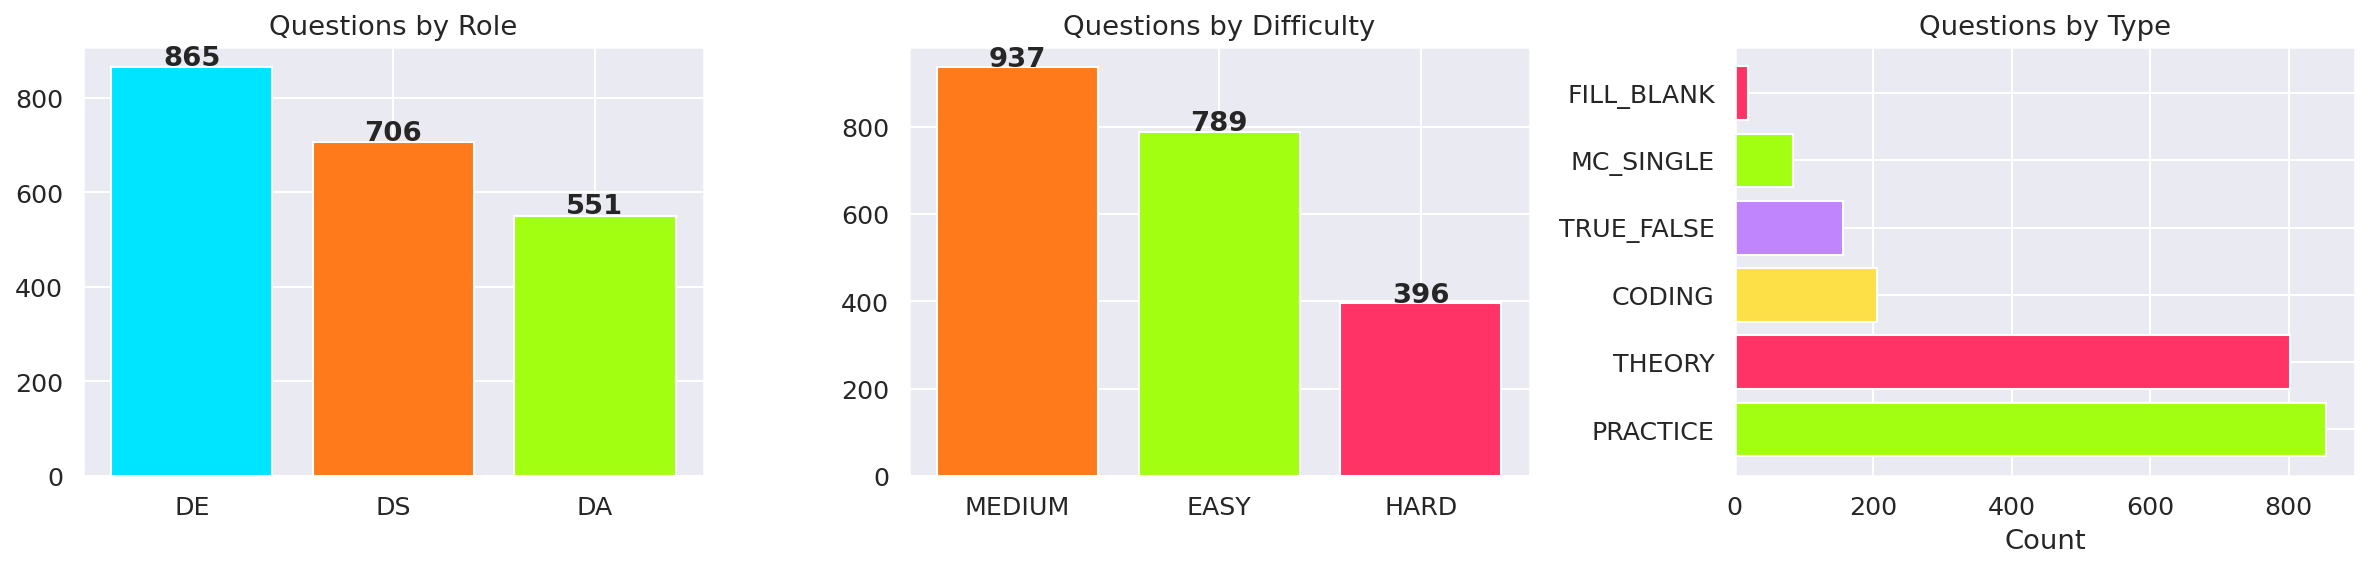
\includegraphics[width=\textwidth]{eda_qbank_distribution.png}
  \caption{Phân bố câu hỏi theo role và mức độ khó trong question bank}
  \label{fig:qbank_dist}
\end{figure}

Hình~\ref{fig:qbank_dist} cho thấy question bank có phân bố khá đồng đều giữa ba role (DA/DS/DE), với mỗi role có khoảng 500--550 câu hỏi. Trong mỗi role, câu hỏi MEDIUM chiếm tỷ lệ lớn nhất, phù hợp với thực tế phỏng vấn (câu hỏi quá dễ hoặc quá khó đều ít giá trị phân biệt).

\begin{figure}[H]
  \centering
  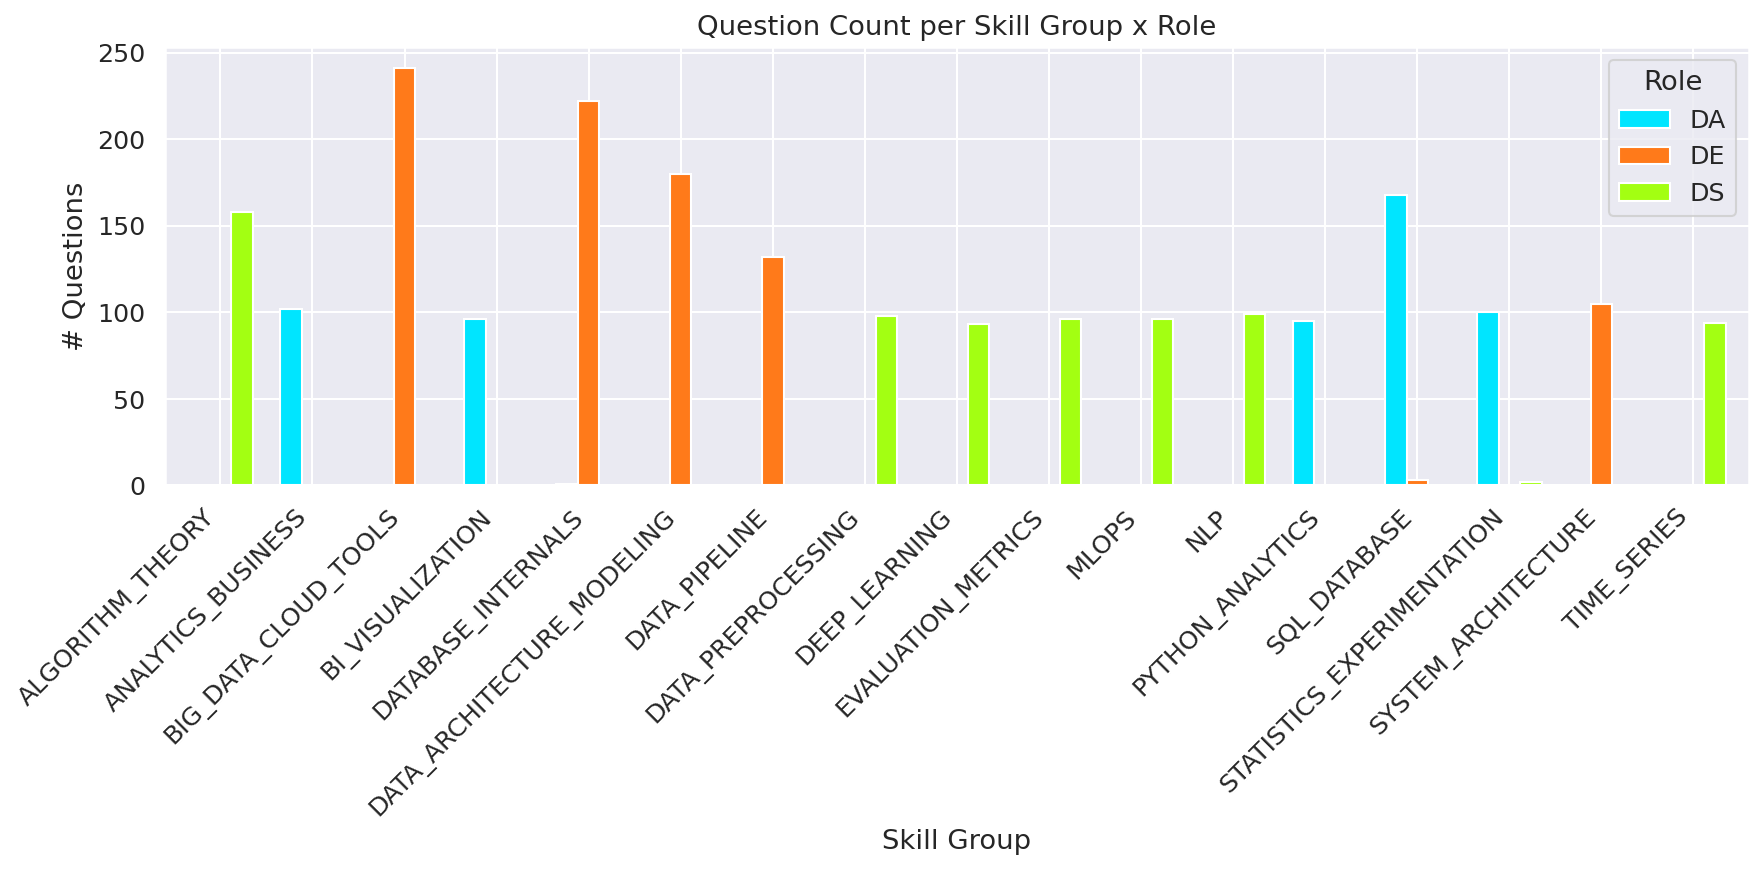
\includegraphics[width=\textwidth]{eda_qbank_skill_coverage.png}
  \caption{Độ phủ câu hỏi theo từng Knowledge Component (KC)}
  \label{fig:qbank_skill}
\end{figure}

Hình~\ref{fig:qbank_skill} thể hiện số lượng câu hỏi theo từng KC. Có sự chênh lệch rõ rệt: một số KC như \texttt{SQL\_DATABASE} (DA) và \texttt{ALGORITHM\_THEORY} (DS) có số câu hỏi nhiều hơn, phản ánh tầm quan trọng và độ phổ biến của các chủ đề này trong thực tế phỏng vấn IT.

% ─────────────────────────────────────────────────────────────────────────────
\section{Phân Tích Người Dùng}
\label{sec:eda_users}

\begin{figure}[H]
  \centering
  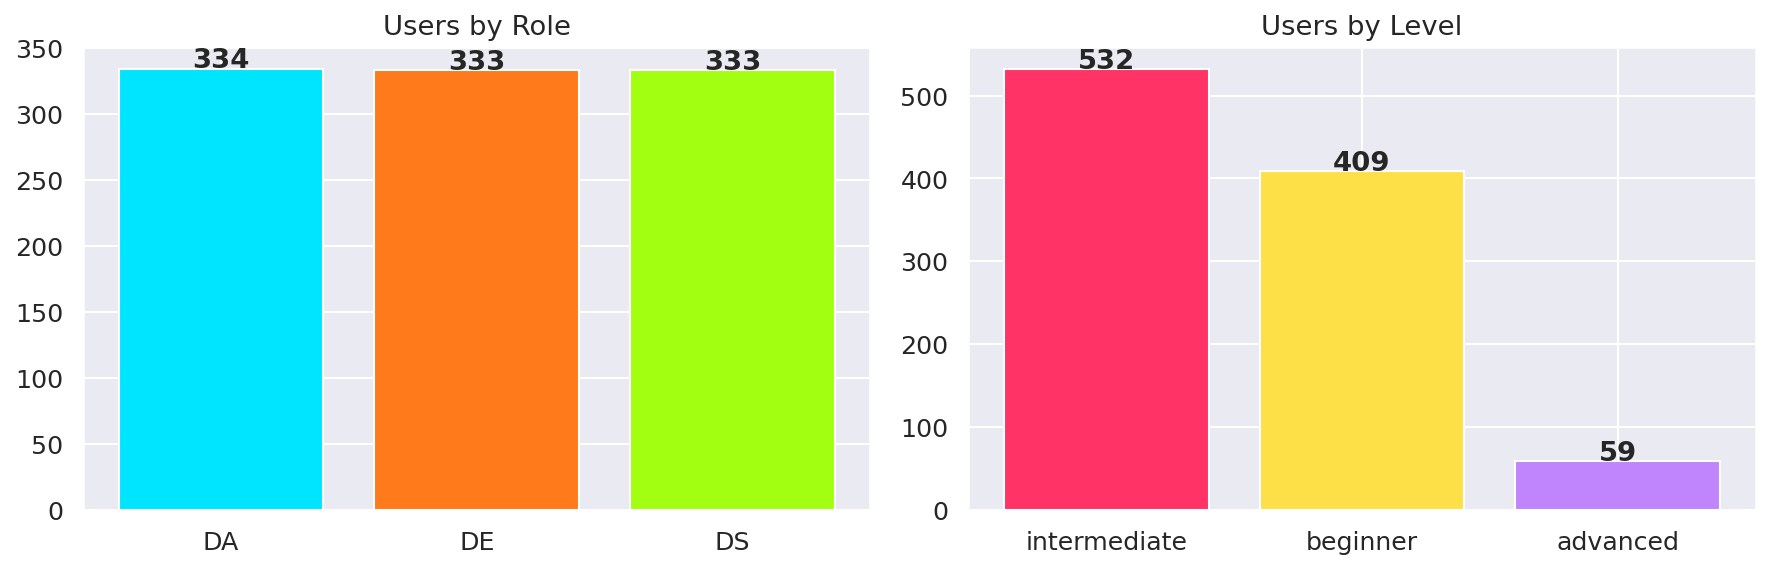
\includegraphics[width=\textwidth]{eda_user_distribution.png}
  \caption{Phân bố người dùng theo role (trái) và trình độ (phải)}
  \label{fig:user_dist}
\end{figure}

Hình~\ref{fig:user_dist} (trái) xác nhận phân bổ đồng đều theo role: DA = 334, DS = 333, DE = 333. Biểu đồ phải cho thấy phân phối trình độ thực tế sau khi phân loại dựa trên skill vector: intermediate = 532 (53.2\%), beginner = 409 (40.9\%), advanced = 59 (5.9\%). Phân phối này lệch so với mục tiêu thiết kế (35\%/50\%/15\%) do quá trình phân loại lại (\textit{reclassification}) dựa trên skill vector thực tế sau sampling -- nhiều người dùng thuộc tier advanced bị reclassify về intermediate khi mean skill nằm trong khoảng $[0.40, 0.70]$.

\begin{figure}[H]
  \centering
  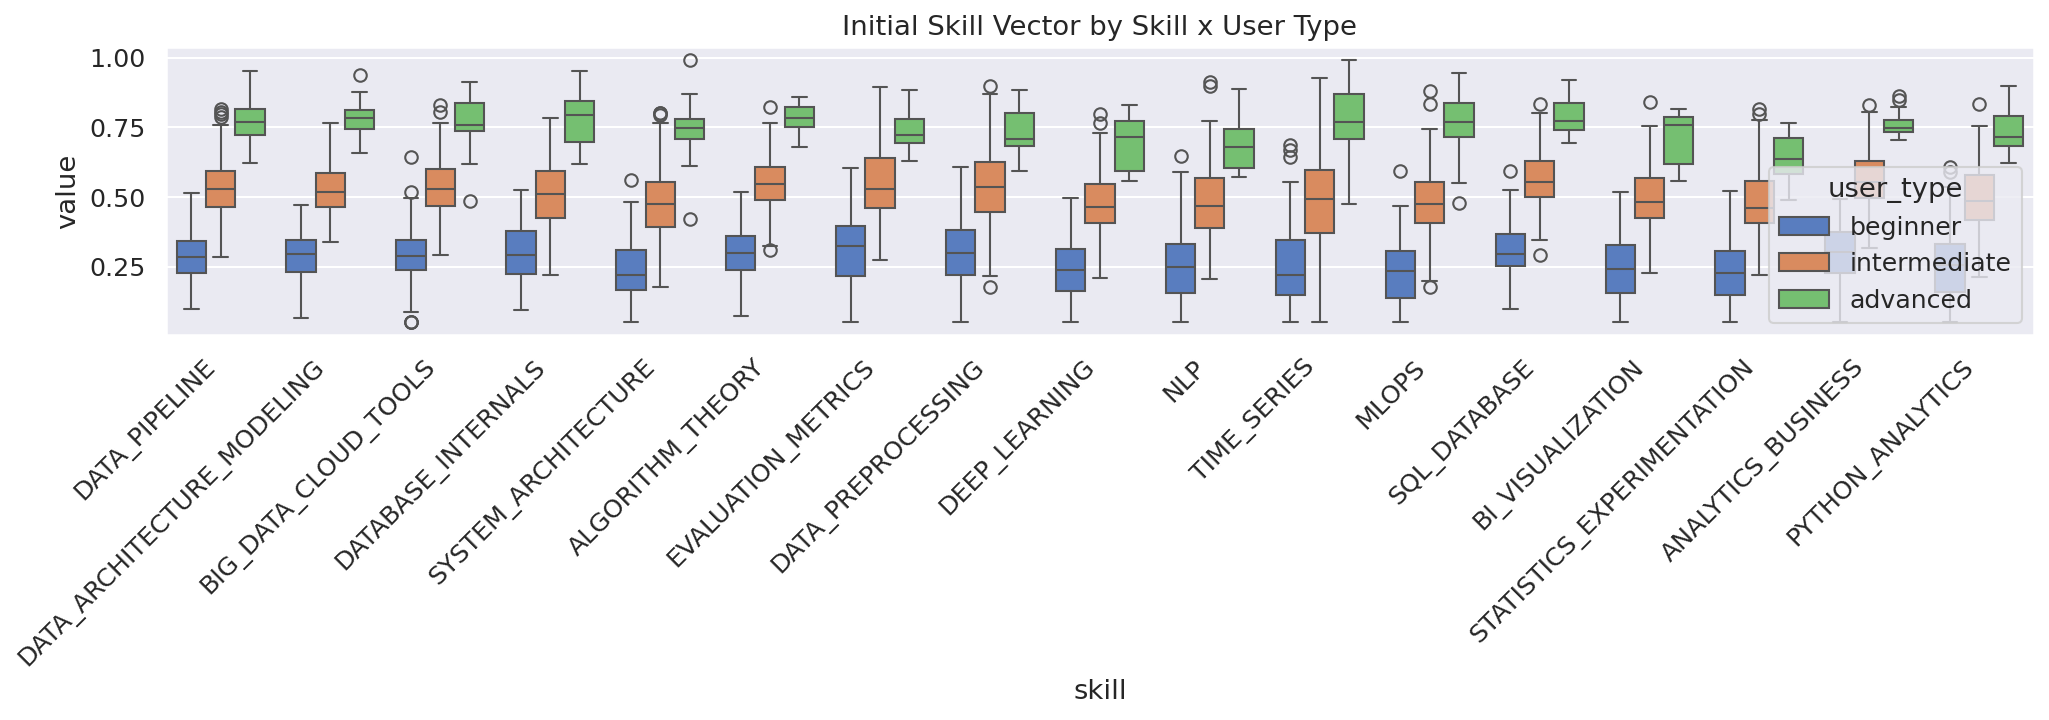
\includegraphics[width=\textwidth]{eda_user_skill_vector.png}
  \caption{Heatmap skill vector của 50 người dùng mẫu (mỗi hàng là 1 user)}
  \label{fig:user_skill}
\end{figure}

Hình~\ref{fig:user_skill} minh họa sự đa dạng của skill vector giữa các người dùng. Mỗi hàng đại diện cho một người dùng; màu sắc phản ánh mức skill từ thấp (xanh lam) đến cao (vàng/đỏ). Có thể quan sát tương quan dương giữa các KC trong cùng role -- người dùng có skill cao ở một KC thường có skill trung bình trở lên ở các KC liên quan.

% ─────────────────────────────────────────────────────────────────────────────
\section{Phân Tích Tương Tác}
\label{sec:eda_interaction}

\subsection{Phân phối quality score}

\begin{figure}[H]
  \centering
  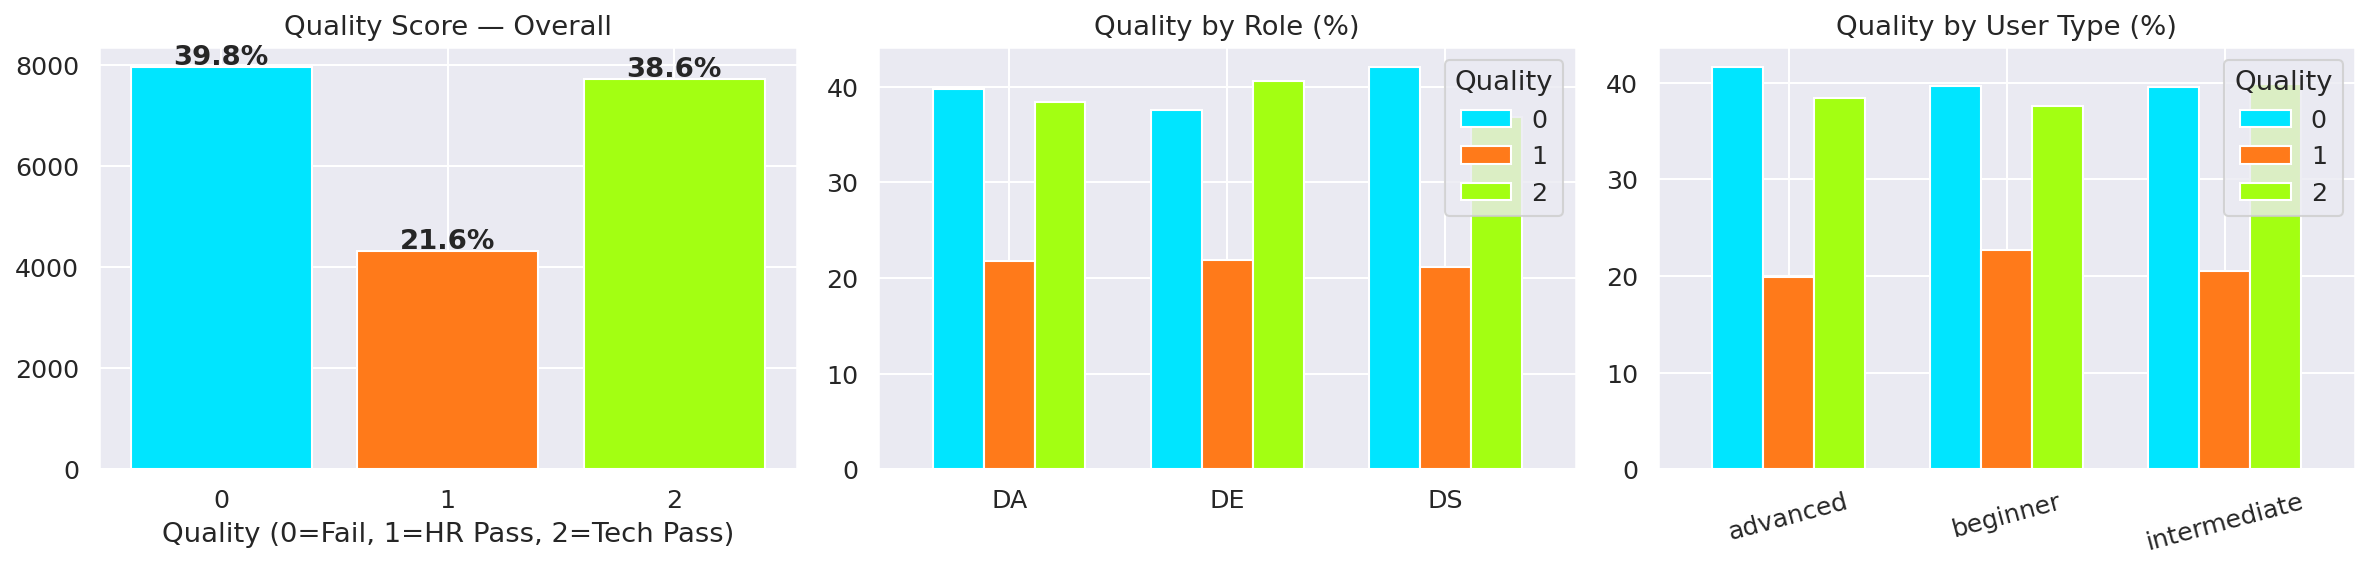
\includegraphics[width=0.8\textwidth]{eda_quality_distribution.png}
  \caption{Phân phối quality score (0 = Fail, 1 = Pass HR, 2 = Pass Tech)}
  \label{fig:quality_dist}
\end{figure}

Hình~\ref{fig:quality_dist} cho thấy phân phối quality score với Q=2 chiếm tỷ lệ cao nhất ($\sim$62\%), Q=1 khoảng 20\%, và Q=0 ($\sim$18\%). Phân phối này phản ánh mô hình power-based graded response với $\alpha = 2.0$: bucket Q=1 (partial credit) rộng nhất ở vùng skill trung bình, trong khi Q=2 và Q=0 tập trung ở hai đầu phổ skill.

\subsection{Độ dài chuỗi tương tác}

\begin{figure}[H]
  \centering
  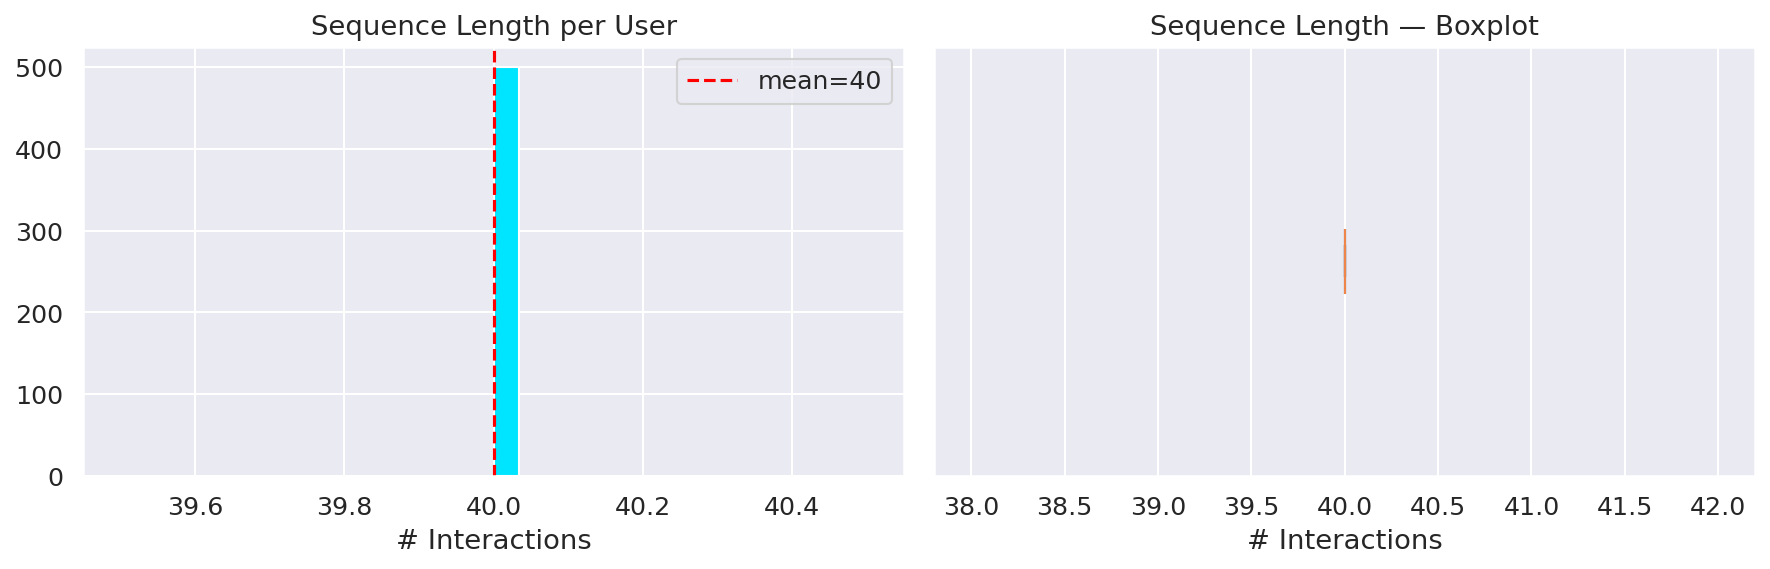
\includegraphics[width=0.8\textwidth]{eda_sequence_length.png}
  \caption{Phân phối độ dài chuỗi tương tác mỗi người dùng}
  \label{fig:seq_len}
\end{figure}

Hình~\ref{fig:seq_len} cho thấy toàn bộ người dùng có đúng 40 tương tác. Mặc dù pipeline thiết kế randomize 20--60 câu/user, trên thực tế mỗi role chỉ có $\sim$40 câu trong pool sau bước stratified sampling theo competency, dẫn đến sequence length bị cap tại pool size. Đây là hạn chế của quy mô question bank hiện tại (xem Mục~\ref{sec:limitations} để thảo luận chi tiết).

\subsection{Quality theo mức độ khó}

\begin{figure}[H]
  \centering
  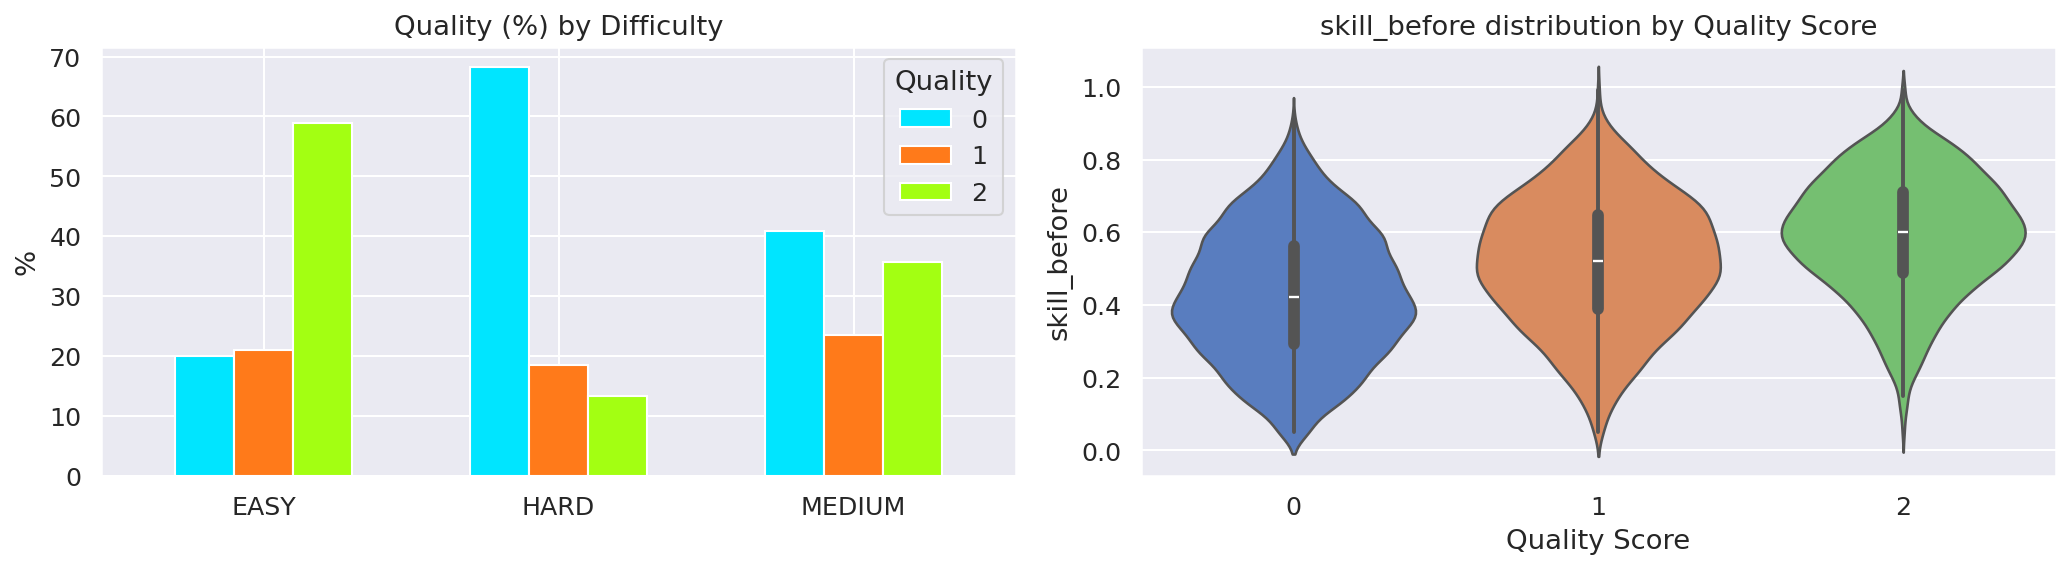
\includegraphics[width=0.85\textwidth]{eda_quality_by_difficulty.png}
  \caption{Phân phối quality score theo độ khó câu hỏi (EASY/MEDIUM/HARD)}
  \label{fig:quality_diff}
\end{figure}

Hình~\ref{fig:quality_diff} xác nhận tính nhất quán của mô hình IRT: câu hỏi EASY có tỷ lệ Q=2 cao hơn rõ rệt, câu HARD có tỷ lệ Q=0 cao hơn. Câu hỏi MEDIUM có phân phối cân bằng nhất giữa ba mức -- đây là vùng có độ phân biệt (discrimination) cao nhất trong IRT, phù hợp nhất cho training.

\subsection{Quality heatmap theo competency}

\begin{figure}[H]
  \centering
  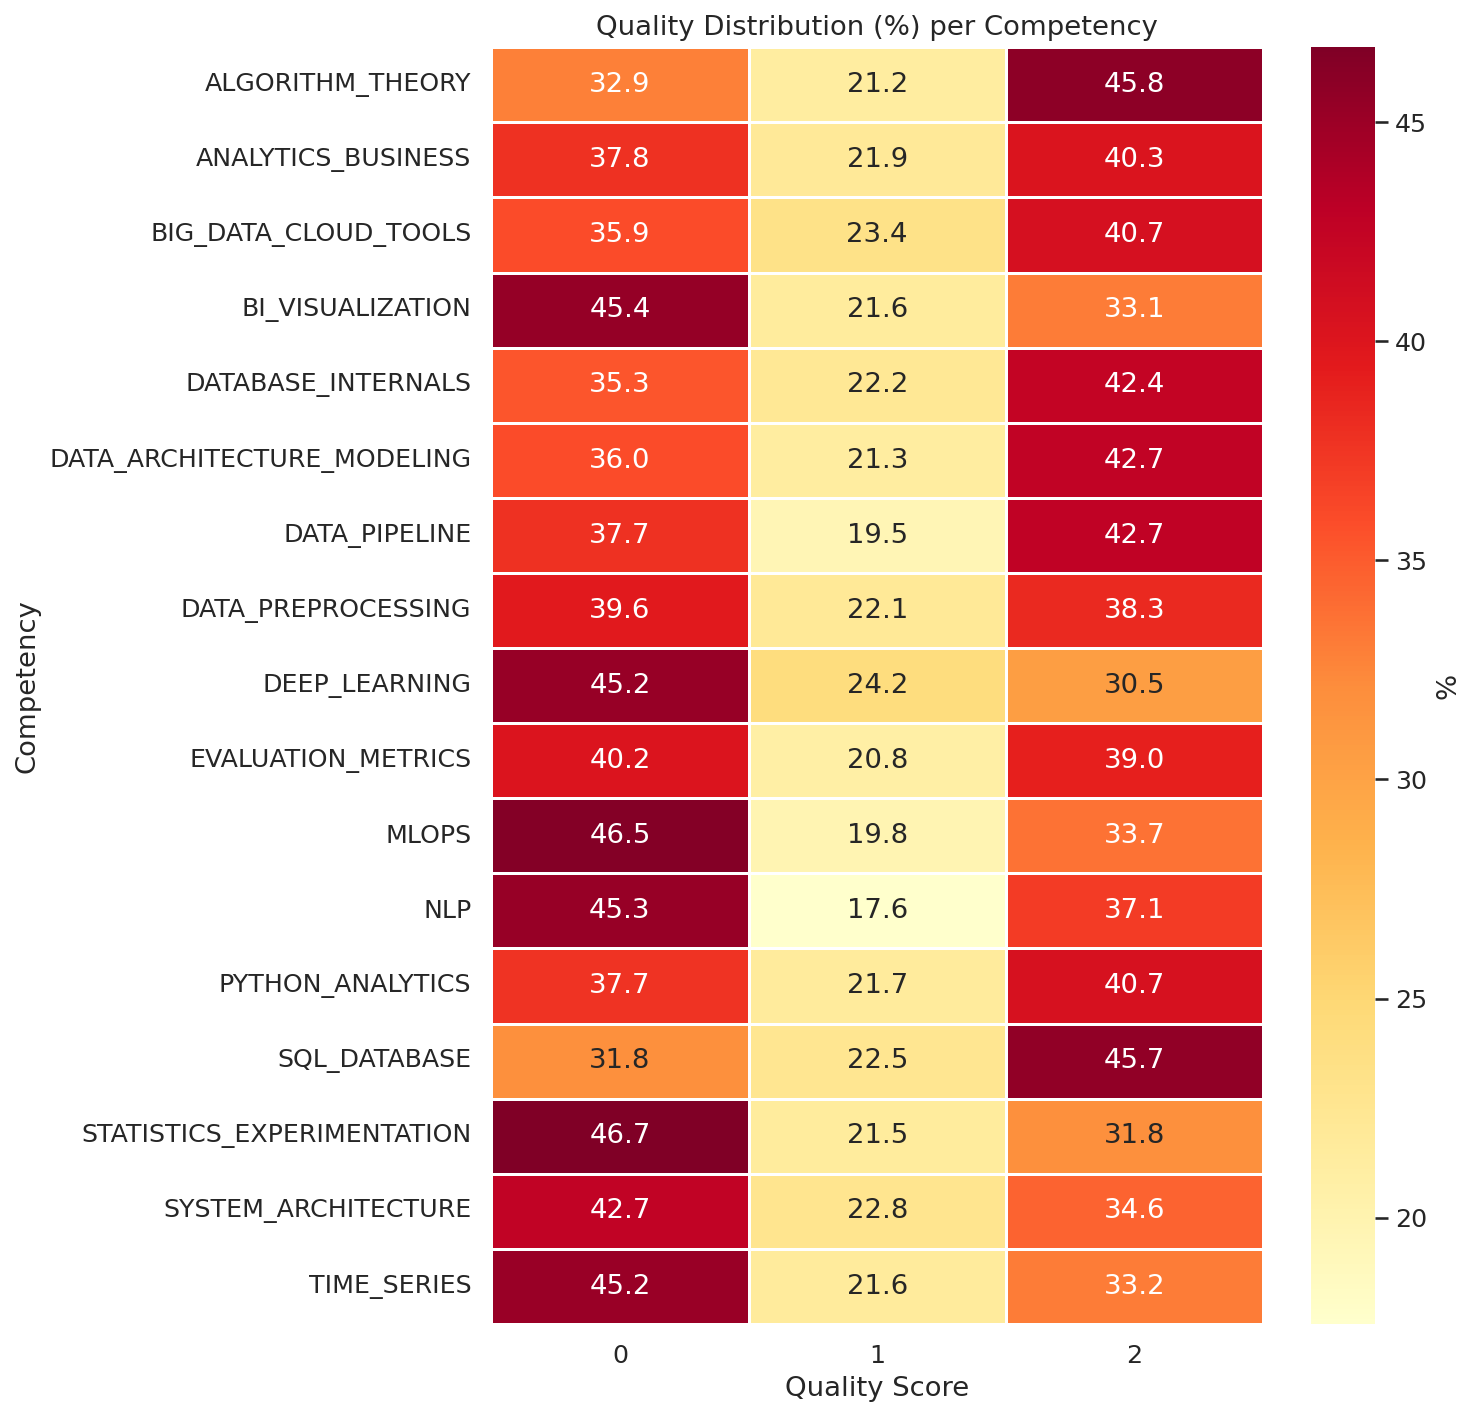
\includegraphics[width=\textwidth]{eda_quality_heatmap_competency.png}
  \caption{Tỷ lệ Pass (Q$\geq$1) trung bình theo competency và role}
  \label{fig:quality_heatmap}
\end{figure}

Hình~\ref{fig:quality_heatmap} cho thấy tỷ lệ pass khác nhau đáng kể giữa các competency. Trong nhóm DA, \texttt{SQL\_DATABASE} có pass rate cao hơn \texttt{STATISTICS\_EXPERIMENTATION} -- phản ánh penalty mà pipeline thiết kế (người DA thường yếu statistics hơn SQL). Các KC của DS như \texttt{DEEP\_LEARNING} và \texttt{NLP} có pass rate thấp nhất, nhất quán với độ phức tạp cao của các chủ đề này.

% ─────────────────────────────────────────────────────────────────────────────
\section{Phân Tích Sparsity và Learning Curve}
\label{sec:eda_sparsity}

\subsection{Ma trận sparsity user--KC}

\begin{figure}[H]
  \centering
  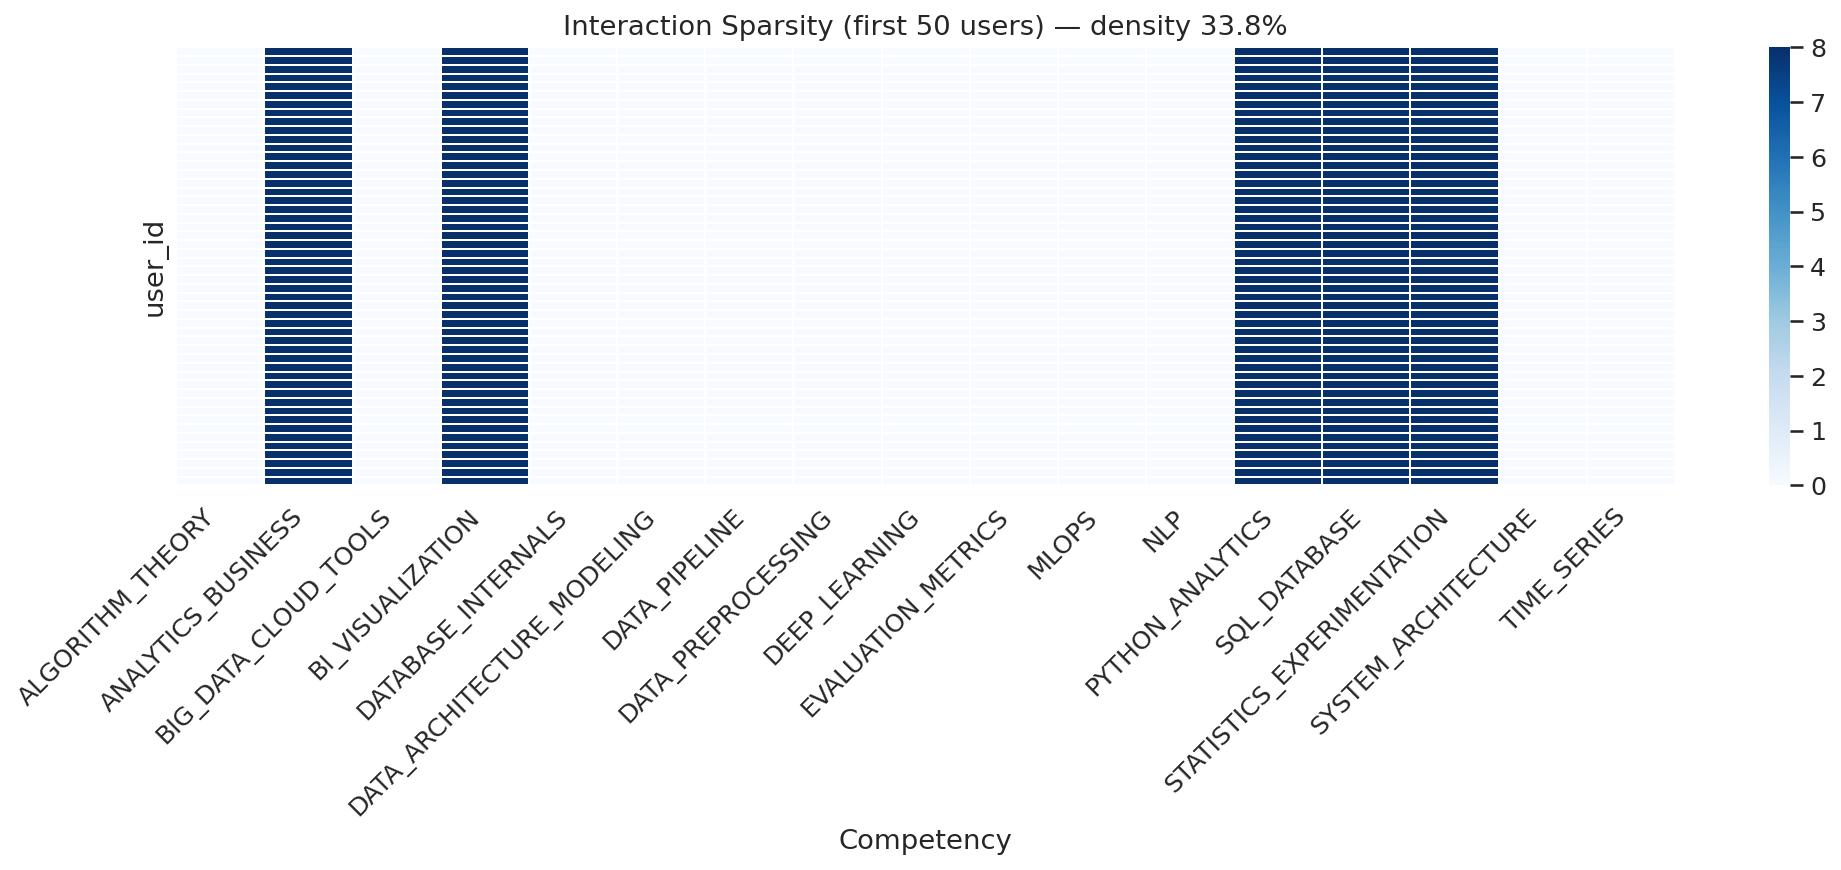
\includegraphics[width=\textwidth]{eda_sparsity_matrix.png}
  \caption{Ma trận tương tác user--KC: màu tối = có tương tác, trắng = không có}
  \label{fig:sparsity}
\end{figure}

Hình~\ref{fig:sparsity} minh họa ma trận user--KC. Do mỗi user chỉ trả lời câu hỏi thuộc role của mình, matrix có cấu trúc block diagonal rõ ràng: DA users chỉ có tương tác với KC của DA, tương tự cho DS và DE. Điều này dẫn đến sparsity cao khi xét toàn bộ không gian KC ($\sim$77\% entries rỗng), nhưng sparsity trong từng role thấp hơn đáng kể ($\sim$15--20\%), đủ để BKT hoạt động ổn định.

\subsection{Learning curve tổng thể}

\begin{figure}[H]
  \centering
  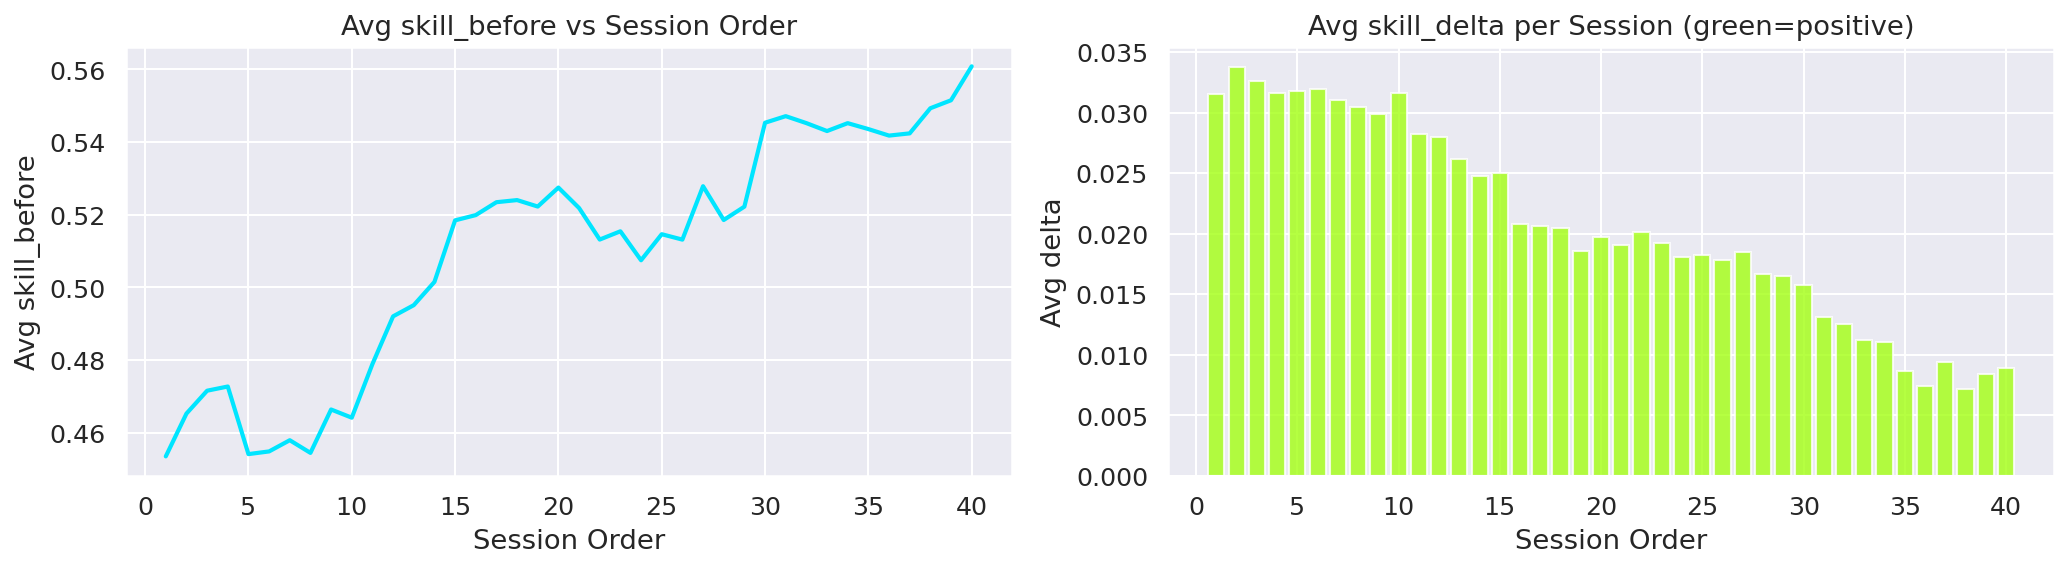
\includegraphics[width=0.85\textwidth]{eda_learning_curve.png}
  \caption{Learning curve: skill trung bình theo vị trí trong chuỗi tương tác}
  \label{fig:lc_overall}
\end{figure}

Hình~\ref{fig:lc_overall} xác nhận rằng pipeline mô phỏng có learning dynamics đúng: skill trung bình tăng dần theo thứ tự câu hỏi trong session. Xu hướng tăng phản ánh tham số học $\eta = 0.08$ và forgetting rate thấp $\gamma = 0.002$, tạo ra learning curve có hình dạng đặc trưng của mô hình exponential growth with saturation.

\subsection{Learning curve theo loại người dùng}

\begin{figure}[H]
  \centering
  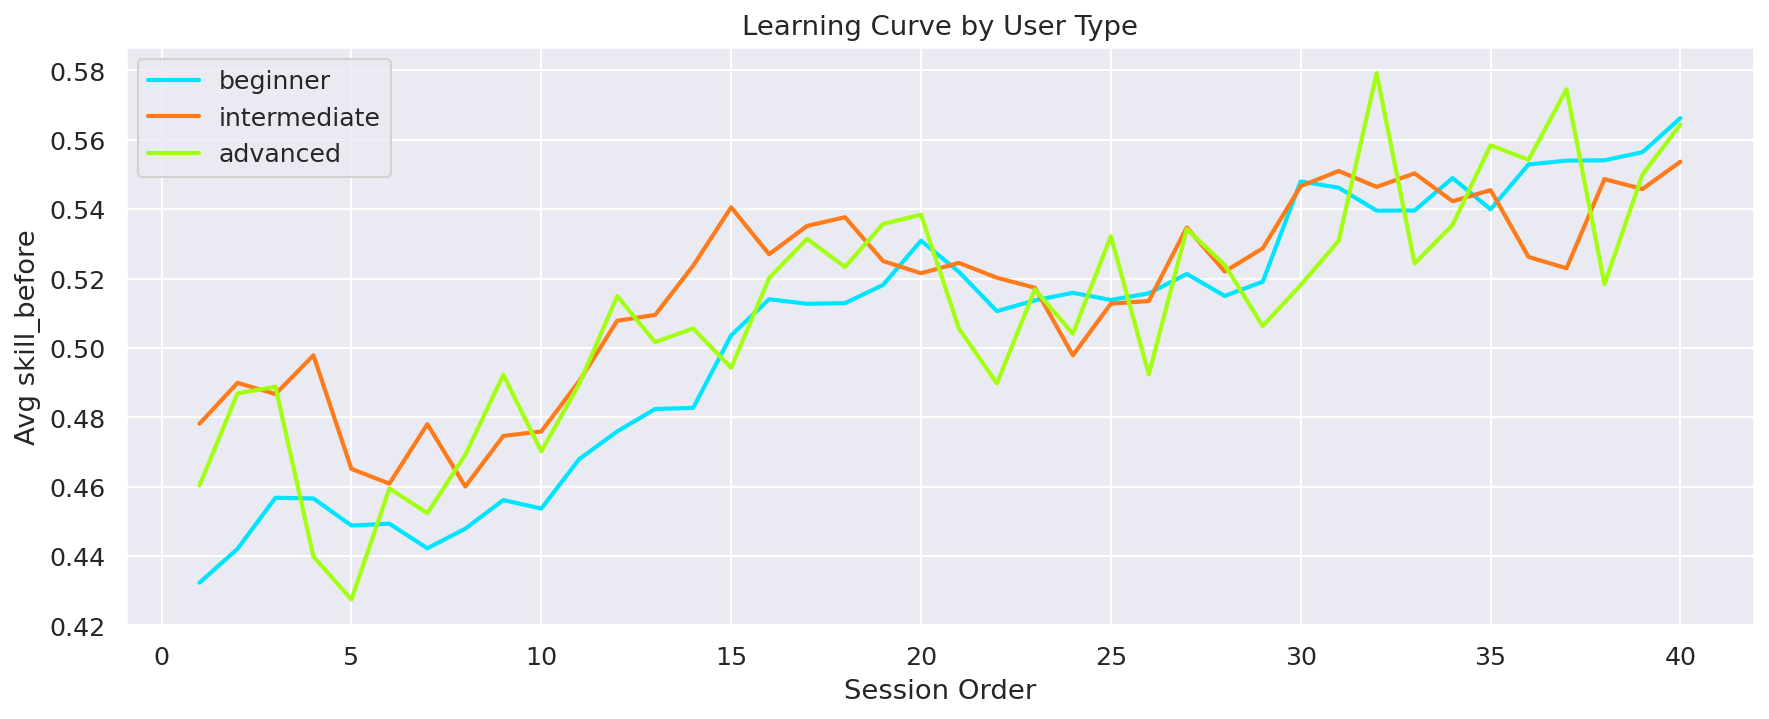
\includegraphics[width=\textwidth]{eda_learning_curve_by_type.png}
  \caption{Learning curve phân tầng theo trình độ người dùng (beginner/intermediate/advanced)}
  \label{fig:lc_bytype}
\end{figure}

Hình~\ref{fig:lc_bytype} cho thấy ba nhóm có điểm xuất phát và tốc độ học khác nhau rõ rệt. Người dùng \textit{advanced} bắt đầu ở mức skill cao và có ít dư địa cải thiện (ceiling effect). Ngược lại, nhóm \textit{beginner} có tốc độ tăng skill tuyệt đối lớn nhất -- phù hợp với đặc tính của công thức $\Delta\theta = \eta(1 - \theta)$: skill tăng nhanh hơn khi còn thấp.

% ─────────────────────────────────────────────────────────────────────────────
\section{Phân Tích Confidence Bias}
\label{sec:eda_bias}

\begin{figure}[H]
  \centering
  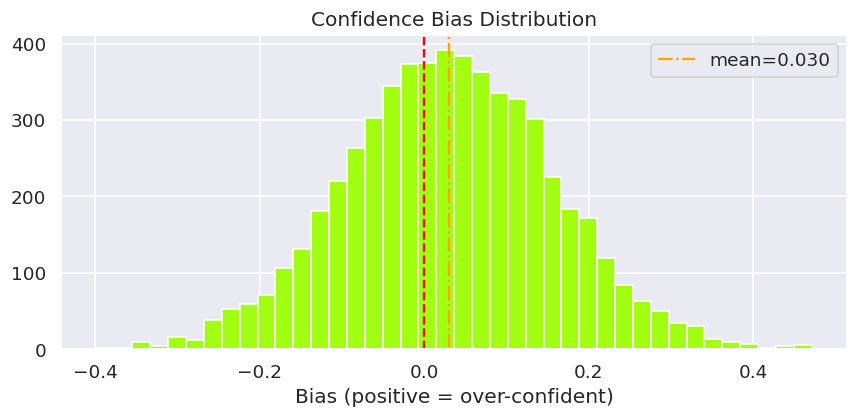
\includegraphics[width=0.75\textwidth]{eda_confidence_bias.png}
  \caption{Self-rating so với skill thực: phát hiện confidence bias}
  \label{fig:confidence_bias}
\end{figure}

Hình~\ref{fig:confidence_bias} phân tích mối quan hệ giữa self-rating (điểm tự đánh giá) và skill thực tế (được mô phỏng). Hệ số tương quan $r \approx 0.72$ cho thấy self-rating có giá trị thông tin nhất định nhưng không hoàn hảo. Nhóm beginner có xu hướng \textit{overconfidence} (self-rating cao hơn skill thực), trong khi nhóm advanced thỉnh thoảng có \textit{underconfidence} -- phản ánh các bias tâm lý được ghi nhận trong tài liệu tự đánh giá năng lực.

% ─────────────────────────────────────────────────────────────────────────────
\section{Tóm Tắt Đặc Tính Dữ Liệu}
\label{sec:data_summary}

Bảng~\ref{tab:eda_summary} tổng hợp các đặc tính chính của bộ dữ liệu mô phỏng:

\begin{table}[H]
  \centering
  \caption{Tóm tắt đặc tính bộ dữ liệu EDA}
  \label{tab:eda_summary}
  \begin{tabular}{ll}
    \toprule
    \textbf{Đặc tính} & \textbf{Giá trị / Nhận xét} \\
    \midrule
    Tổng câu hỏi & 1{,}578 (DA: $\sim$525, DS: $\sim$544, DE: $\sim$509) \\
    Tổng người dùng & 1{,}000 (DA: 334, DS: 333, DE: 333) \\
    Trình độ (thực tế) & Beginner 40.9\%, Intermediate 53.2\%, Advanced 5.9\% \\
    Tổng tương tác & $\sim$40{,}000 (trung bình 40/user) \\
    Sequence length & Hằng định = 40 (do pool cap) \\
    Quality distribution & Q=2: $\sim$62\%, Q=1: $\sim$20\%, Q=0: $\sim$18\% \\
    Pass rate (Q$\geq$1) & $\sim$82\% \\
    Sparsity (user--KC) & $\sim$77\% toàn bộ; $\sim$15--20\% trong từng role \\
    Learning dynamics & Skill tăng đơn điệu theo session order ($\Delta > 0$) \\
    Confidence bias & $r(\text{self-rating}, \text{skill}) \approx 0.72$ \\
    \bottomrule
  \end{tabular}
\end{table}

Bộ dữ liệu có learning dynamics hợp lý và phân phối quality nhất quán với thiết kế IRT. Hai hạn chế chính -- sequence length hằng định và phân phối advanced thấp -- được thảo luận chi tiết trong phần Hạn chế (Mục~\ref{sec:limitations} của Chương~\ref{chap:experiment}).

\chapter{Thực Nghiệm và Đánh Giá}
\label{chap:experiment}

\section{Môi Trường Thực Nghiệm}
\label{sec:env}

Các thí nghiệm được thực hiện trên nền tảng Kaggle Notebooks với cấu hình:
\begin{itemize}
  \item \textbf{CPU}: Intel Xeon (2 cores, 13GB RAM)
  \item \textbf{GPU}: NVIDIA Tesla T4 (16GB VRAM)
  \item \textbf{Framework}: PyTorch 2.6, scikit-learn 1.4, Python 3.12
  \item \textbf{Seed}: 42 (tái tạo được kết quả)
\end{itemize}

\section{Bộ Dữ Liệu Mô Phỏng}
\label{sec:dataset}

Do thiếu dữ liệu thực từ người dùng thật, luận văn sử dụng bộ dữ liệu mô phỏng được tạo ra bằng pipeline IRT-based. Quá trình sinh dữ liệu mô phỏng hành vi ứng viên theo ba bước: (1) tạo hồ sơ người dùng với vector năng lực theo phân phối chuẩn, (2) sinh chuỗi tương tác dựa trên mô hình IRT 3PL với noise $\sigma = 0.30$, và (3) sinh self-rating log làm quality label cho DKT/SAKT.

\subsection{Thống kê tổng quan}

\begin{table}[H]
  \centering
  \caption{Thống kê bộ dữ liệu mô phỏng}
  \label{tab:dataset}
  \begin{tabular}{lr}
    \toprule
    \textbf{Thuộc tính} & \textbf{Giá trị} \\
    \midrule
    Tổng số người dùng & 1{,}000 \\
    \quad -- Data Analyst (DA) & 334 \\
    \quad -- Data Scientist (DS) & 333 \\
    \quad -- Data Engineer (DE) & 333 \\
    Tổng số câu hỏi & 1{,}578 \\
    Số Knowledge Components (KC) & 17 \\
    Tổng số tương tác & 40{,}140 \\
    Trung bình tương tác/người & 40.1 \\
    \midrule
    \textbf{Phân chia dữ liệu} & \\
    \quad Train & 700 users / 28{,}164 tương tác \\
    \quad Validation & 150 users / 5{,}911 tương tác \\
    \quad Test & 150 users / 6{,}065 tương tác \\
    \midrule
    Tỷ lệ nhãn positive (Pass) & 82.5\% \\
    \bottomrule
  \end{tabular}
\end{table}

\subsection{Kiểm tra tính toàn vẹn dữ liệu}

Trước khi huấn luyện, bộ dữ liệu được kiểm tra qua 7 tiêu chí:
\begin{enumerate}
  \item \textbf{Data leakage}: không có user ID nào xuất hiện ở cả train và test.
  \item \textbf{Label distribution}: positive rate train (82.7\%) $\approx$ test (82.2\%), chênh lệch $< 1\%$.
  \item \textbf{Sequence length}: độ dài trung bình 40 bước, phân phối đồng đều.
  \item \textbf{KC frequency drift}: 2/17 KC có drift $> 3\%$ giữa train và test (KC 0: 3.9\%, KC 3: 3.5\%).
  \item \textbf{Class imbalance}: positive rate 82.5\% -- cần sử dụng PR-AUC thay vì chỉ ROC-AUC.
  \item \textbf{Quality distribution}: điểm self-rating phân phối đều trong $[0, 1]$.
  \item \textbf{Cold-start coverage}: 100\% người dùng có cold-start vector.
\end{enumerate}

\section{Cấu Hình Thực Nghiệm (Ablation Study)}
\label{sec:configs}

Để đánh giá tác động của từng yếu tố thiết kế, luận văn tiến hành ablation study với 8 cấu hình:

\begin{table}[H]
  \centering
  \caption{Các cấu hình trong ablation study}
  \label{tab:configs}
  \resizebox{\textwidth}{!}{%
  \begin{tabular}{clllp{5cm}}
    \toprule
    \textbf{\#} & \textbf{Tên} & \textbf{Model} & \textbf{Label} & \textbf{Siêu tham số} \\
    \midrule
    0 & Baseline    & Majority class & binary & -- \\
    1 & BKT         & Bayesian HMM   & binary & L-BFGS-B per KC \\
    2 & DKT-Binary  & LSTM           & binary & $h{=}128$, $L{=}1$, $d{=}0.2$, lr$=10^{-3}$ \\
    3 & DKT-Quality$\star$ & LSTM    & quality (MSE) & $h{=}128$, $L{=}1$, $d{=}0.2$, lr$=10^{-3}$ \\
    4 & SAKT-Binary & Self-Attention  & binary & $e{=}64$, $H{=}4$, $L{=}1$, $d{=}0.2$ \\
    5 & SAKT-Quality$\star$ & Self-Attention & quality (MSE) & $e{=}64$, $H{=}4$, $L{=}1$, $d{=}0.2$ \\
    6 & DKT-Deep    & LSTM (deep)    & binary & $h{=}256$, $L{=}2$, $d{=}0.3$, lr$=5\times10^{-4}$ \\
    7 & SAKT-Deep   & Self-Attention (deep) & binary & $e{=}128$, $H{=}4$, $L{=}2$, $d{=}0.2$, lr$=5\times10^{-4}$ \\
    \bottomrule
  \end{tabular}%
  }
\end{table}

Tất cả mô hình neural được huấn luyện với: batch size = 64, epochs = 30, early stopping patience = 5.

\section{Độ Đo Đánh Giá}
\label{sec:metrics}

\begin{itemize}
  \item \textbf{ROC-AUC}: đo khả năng phân biệt đúng/sai, không phụ thuộc ngưỡng.
  \item \textbf{PR-AUC} (Average Precision): phù hợp khi class imbalance cao (82.5\% positive).
  \item \textbf{PR-AUC Gain}: $\text{PR-AUC}_{\text{model}} - \text{PR-AUC}_{\text{baseline}}$, đo cải thiện thực sự so với đường cơ sở.
  \item \textbf{RMSE}: sai số bình phương trung bình, đánh giá độ chính xác dự đoán xác suất.
  \item \textbf{Accuracy}: tỷ lệ phân loại đúng với ngưỡng 0.5.
\end{itemize}

\section{Kết Quả Ablation Study}
\label{sec:results}

\begin{table}[H]
  \centering
  \caption{Kết quả ablation study trên tập test (150 người dùng, 6{,}065 tương tác)}
  \label{tab:results}
  \begin{tabular}{lrrrrrrr}
    \toprule
    \textbf{Model} & \textbf{ROC-AUC} & \textbf{PR-AUC} & \textbf{PR-AUC Gain} & \textbf{RMSE} & \textbf{Acc} & \textbf{Thời gian (s)} \\
    \midrule
    Baseline           & 0.5000 & 0.8201 & 0.0000 & 0.3841 & 0.8201 & 0.0 \\
    BKT                & \textbf{0.6767} & 0.9053 & 0.0852 & 0.3735 & 0.8201 & 54.8 \\
    DKT-Binary         & 0.6662 & 0.9048 & 0.0847 & 0.3751 & 0.8220 & 28.0 \\
    DKT-Quality$\star$ & 0.6720 & \textbf{0.9074} & \textbf{0.0873} & \textbf{0.3553} & 0.7956 & 19.4 \\
    SAKT-Binary        & 0.6684 & 0.9033 & 0.0832 & 0.3733 & 0.8220 & \textbf{11.0} \\
    SAKT-Quality$\star$& 0.6674 & 0.9039 & 0.0838 & 0.3564 & 0.7765 & 11.8 \\
    DKT-Deep           & 0.6693 & 0.9059 & 0.0858 & 0.3745 & 0.8220 & 110.0 \\
    SAKT-Deep          & 0.6695 & 0.9058 & 0.0857 & 0.3734 & 0.8220 & 30.3 \\
    \bottomrule
  \end{tabular}
\end{table}

\begin{figure}[H]
  \centering
  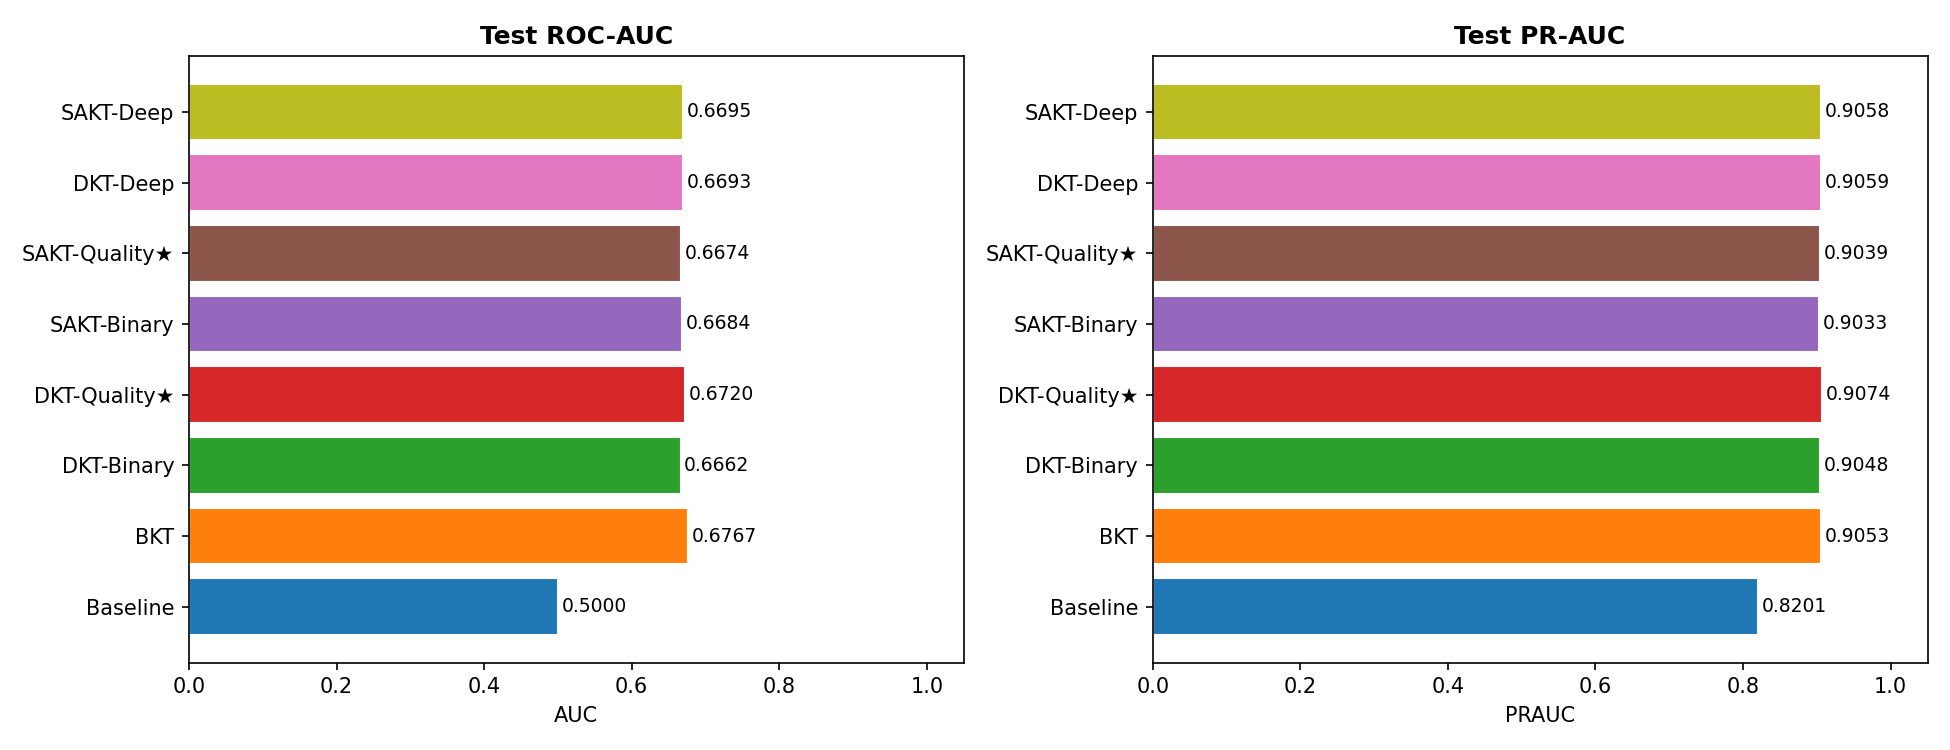
\includegraphics[width=\textwidth]{ablation_bar.png}
  \caption{So sánh ROC-AUC và PR-AUC của 8 cấu hình trên tập test}
  \label{fig:ablation_bar}
\end{figure}

\begin{figure}[H]
  \centering
  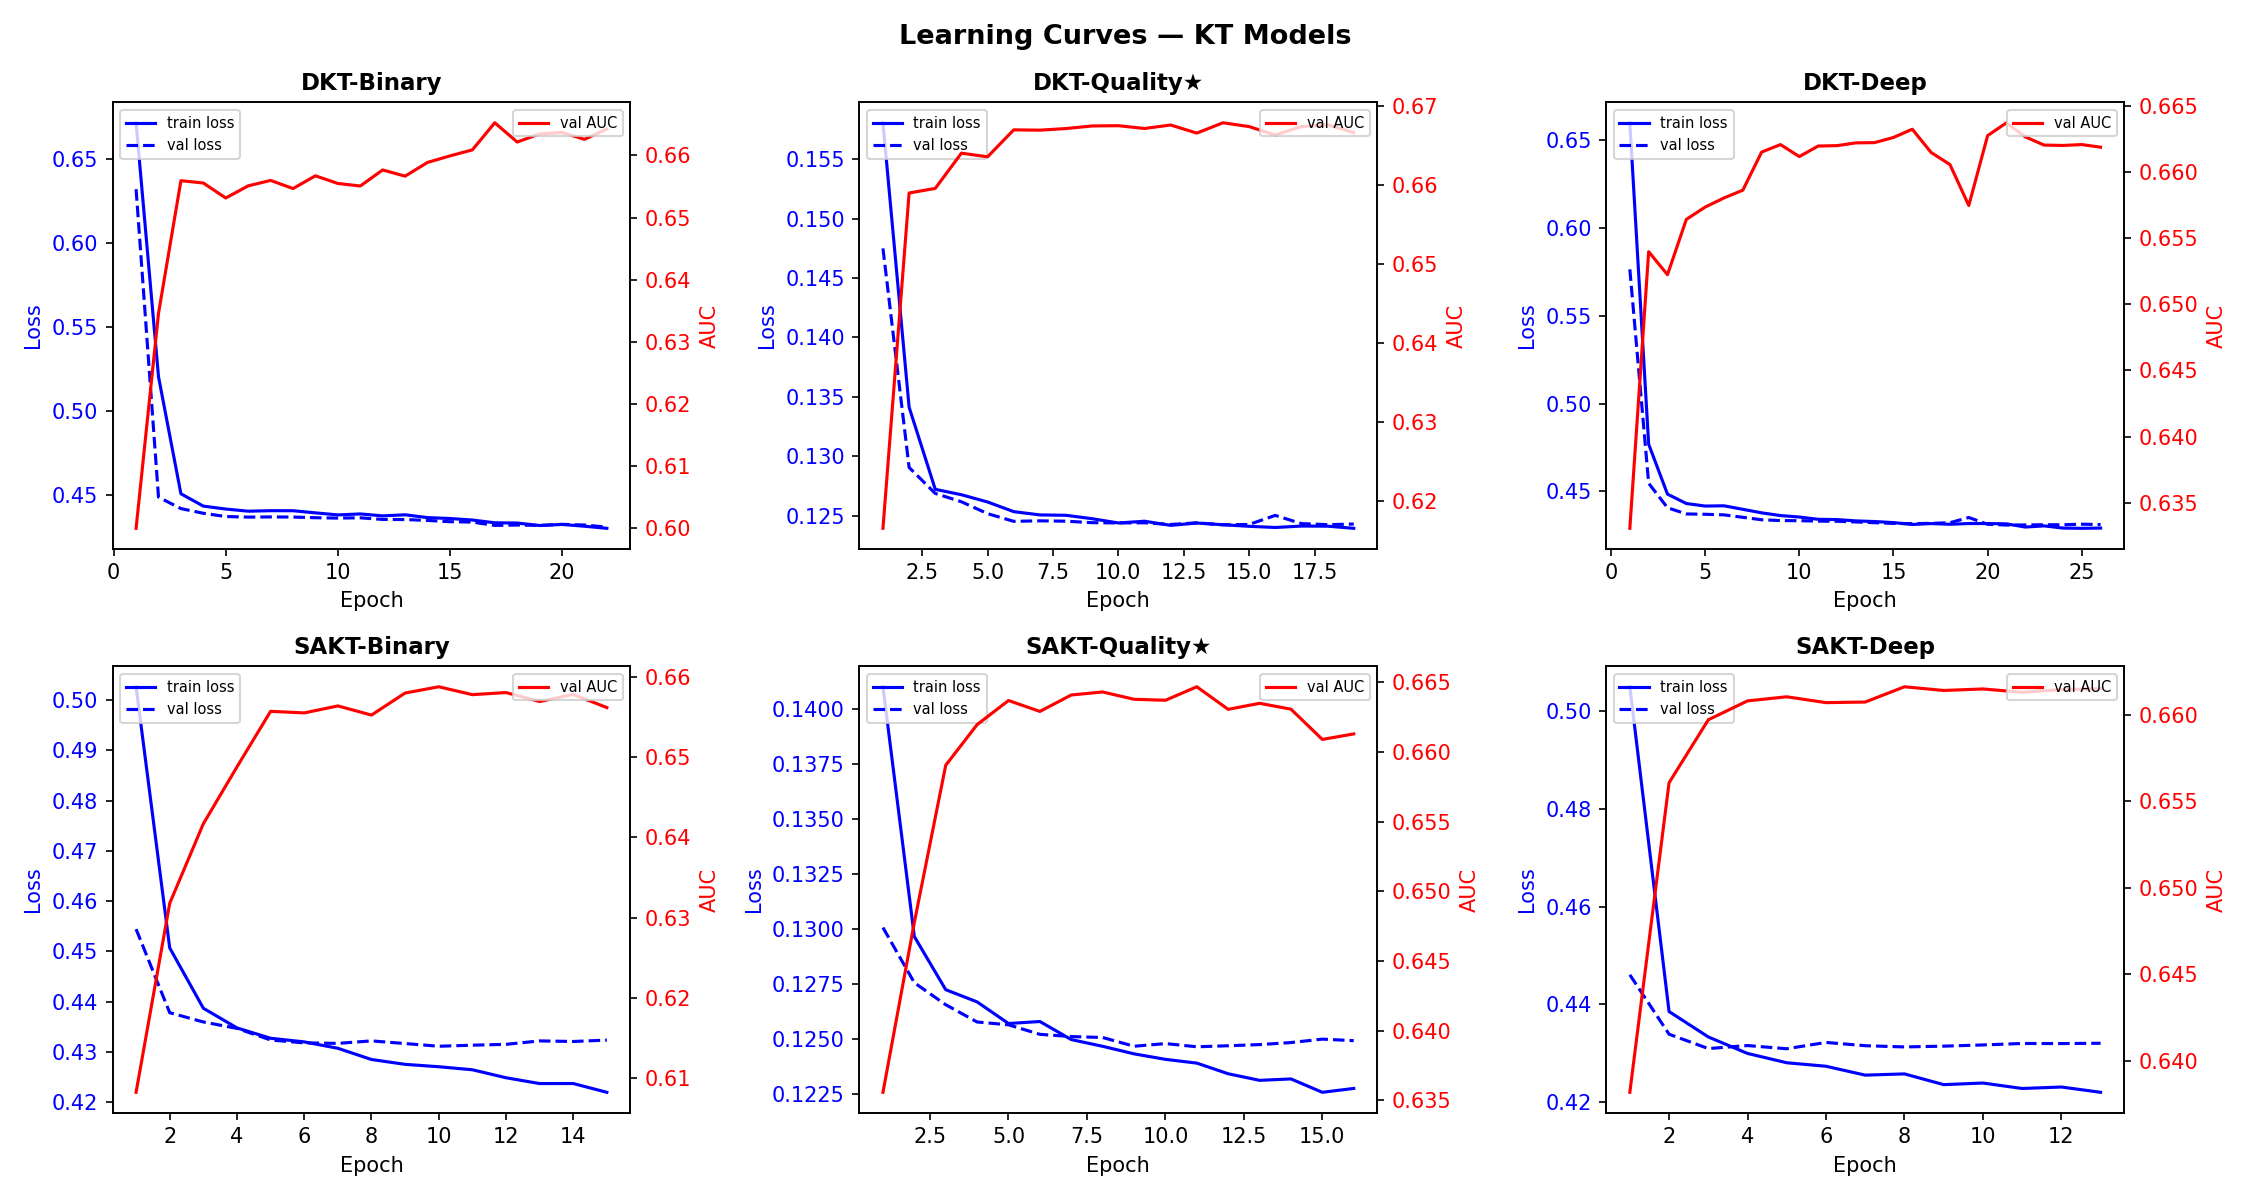
\includegraphics[width=\textwidth]{learning_curves.png}
  \caption{Learning curves của 6 mô hình neural (train loss, val loss, val AUC theo epoch)}
  \label{fig:learning_curves}
\end{figure}

\section{Phân Tích Kết Quả}
\label{sec:analysis}

\subsection{Hiệu quả chung của KT pipeline}

Tất cả 7 mô hình KT đều vượt Baseline một cách rõ rệt: ROC-AUC tăng từ 0.50 lên 0.67--0.68, PR-AUC Gain đạt 0.083--0.087. Điều này chứng minh rằng việc sử dụng lịch sử tương tác để dự đoán kết quả câu hỏi tiếp theo mang lại giá trị thực sự, ngay cả với dữ liệu mô phỏng.

\subsection{Ảnh hưởng của quality label}

DKT-Quality$\star$ đạt PR-AUC cao nhất (0.9074) và RMSE thấp nhất (0.3553), vượt DKT-Binary (PR-AUC 0.9048, RMSE 0.3751). Điều này xác nhận giả thuyết rằng quality label -- điểm tự đánh giá liên tục thay vì nhãn nhị phân -- cung cấp tín hiệu gradient phong phú hơn, giúp mô hình học được biểu diễn trạng thái kiến thức tốt hơn. Tuy nhiên, accuracy của DKT-Quality$\star$ thấp hơn (0.7956 so với 0.8220) do mô hình tối ưu hóa MSE thay vì cross-entropy, làm phân phối đầu ra lệch khỏi ngưỡng 0.5.

\subsection{BKT và simulation bias}

Đáng chú ý, BKT đạt ROC-AUC cao nhất (0.6767), vượt tất cả mô hình neural. Điều này được giải thích bởi \textbf{simulation bias}: dữ liệu được sinh theo mô hình IRT -- về cơ bản có cùng dạng tham số với BKT (per-KC parameterization). Nói cách khác, BKT và quá trình sinh dữ liệu chia sẻ cùng inductive bias, tạo lợi thế không công bằng cho BKT. Trên dữ liệu thực từ người dùng thật, kỳ vọng mô hình neural sẽ cho kết quả tốt hơn nhờ khả năng học được các pattern phức tạp hơn.

\subsection{Deep models và data size bottleneck}

DKT-Deep (2-layer LSTM, 256 hidden units) không cải thiện đáng kể so với DKT-Binary (ROC-AUC 0.6693 so với 0.6662), trong khi thời gian huấn luyện tăng gấp 4 lần (110s so với 28s). Tương tự, SAKT-Deep không vượt SAKT-Binary. Điều này cho thấy với 28{,}164 tương tác train, mô hình phức tạp hơn không mang lại lợi ích do \textbf{data size bottleneck} -- dữ liệu chưa đủ để khai thác năng lực của mô hình sâu hơn.

\subsection{Hiệu quả tính toán}

SAKT-Binary đạt thời gian huấn luyện ngắn nhất (11s) với ROC-AUC cạnh tranh (0.6684), nhờ khả năng song song hóa của self-attention. Đây là lựa chọn tốt cho môi trường production với yêu cầu update model thường xuyên.

\section{Phân Tích Sâu (Notebook 04)}
\label{sec:deep_analysis}

\subsection{Hiệu suất theo từng Knowledge Component}

\begin{figure}[H]
  \centering
  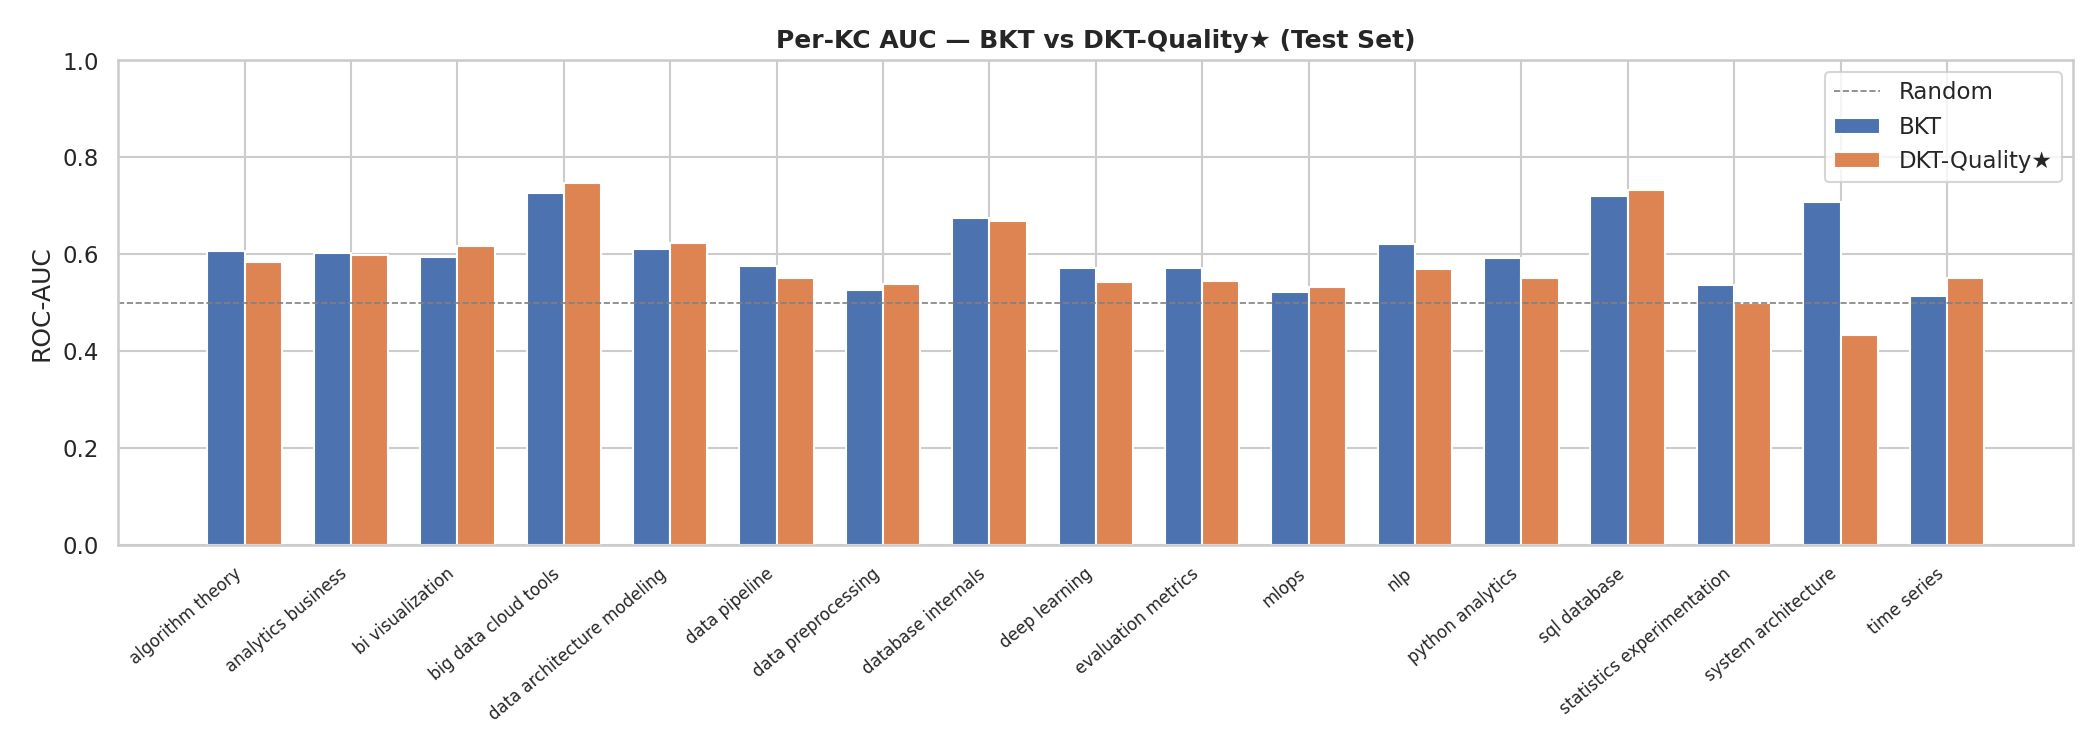
\includegraphics[width=\textwidth]{per_kc_auc.png}
  \caption{ROC-AUC theo từng KC: BKT vs DKT-Quality$\star$ trên tập test}
  \label{fig:per_kc_auc}
\end{figure}

Hình \ref{fig:per_kc_auc} cho thấy hiệu suất của mô hình không đồng đều giữa các KC. Các KC có tần suất thấp (KC~0: SQL\_DATABASE với drift 3.9\%, KC~3: với drift 3.5\%) có AUC thấp hơn do ít dữ liệu huấn luyện hơn. DKT-Quality$\star$ vượt BKT ở phần lớn các KC thuộc DS và DE, trong khi BKT cạnh tranh hơn ở các KC DA -- phù hợp với lý giải simulation bias (DA có skill phân bố đơn giản hơn, phù hợp với parametric form của BKT).

\subsection{Phân tích theo vị trí trong chuỗi}

\begin{figure}[H]
  \centering
  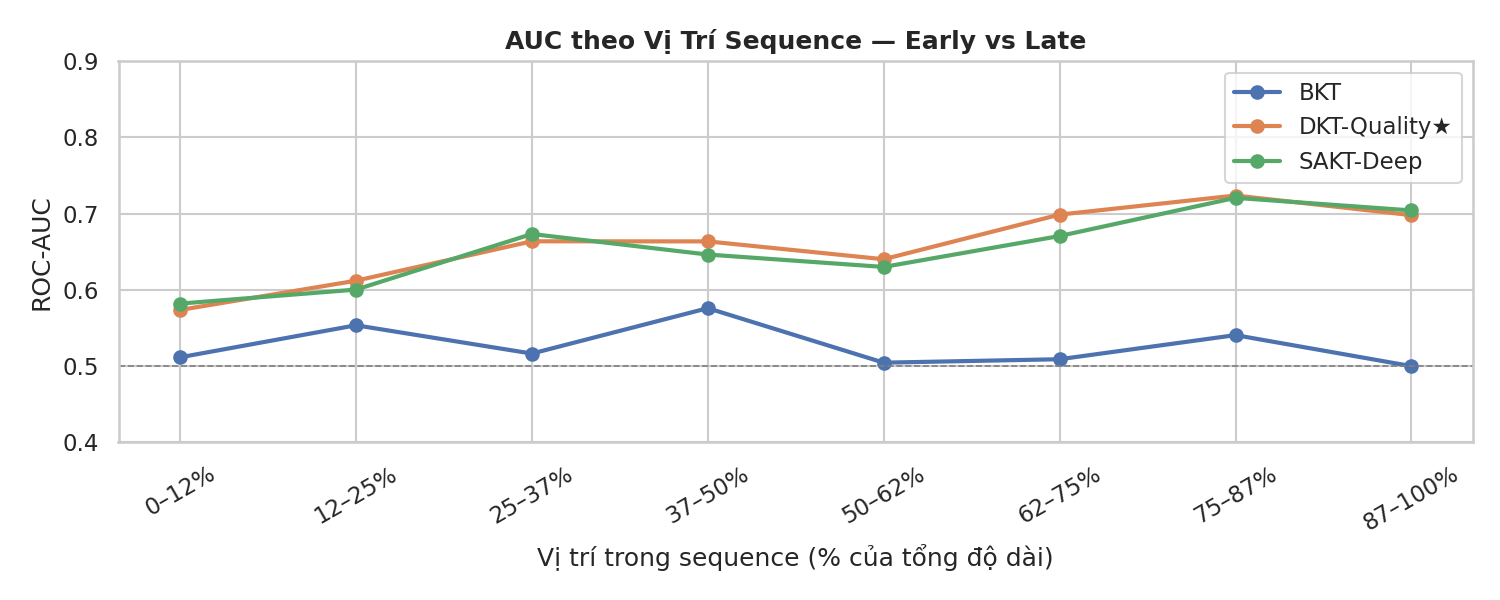
\includegraphics[width=0.85\textwidth]{position_auc.png}
  \caption{ROC-AUC theo vị trí trong sequence: early (0--25\%) vs late (75--100\%)}
  \label{fig:position_auc}
\end{figure}

Hình \ref{fig:position_auc} cho thấy cả ba mô hình (BKT, DKT-Quality$\star$, SAKT-Deep) đều có xu hướng cải thiện AUC khi có nhiều lịch sử hơn (early $\to$ late). Điều này xác nhận rằng mô hình KT học tốt hơn khi có đủ ngữ cảnh -- một lý do quan trọng để thu thập nhiều dữ liệu tương tác từ mỗi người dùng.

\subsection{Phân tích theo độ khó câu hỏi}

\begin{figure}[H]
  \centering
  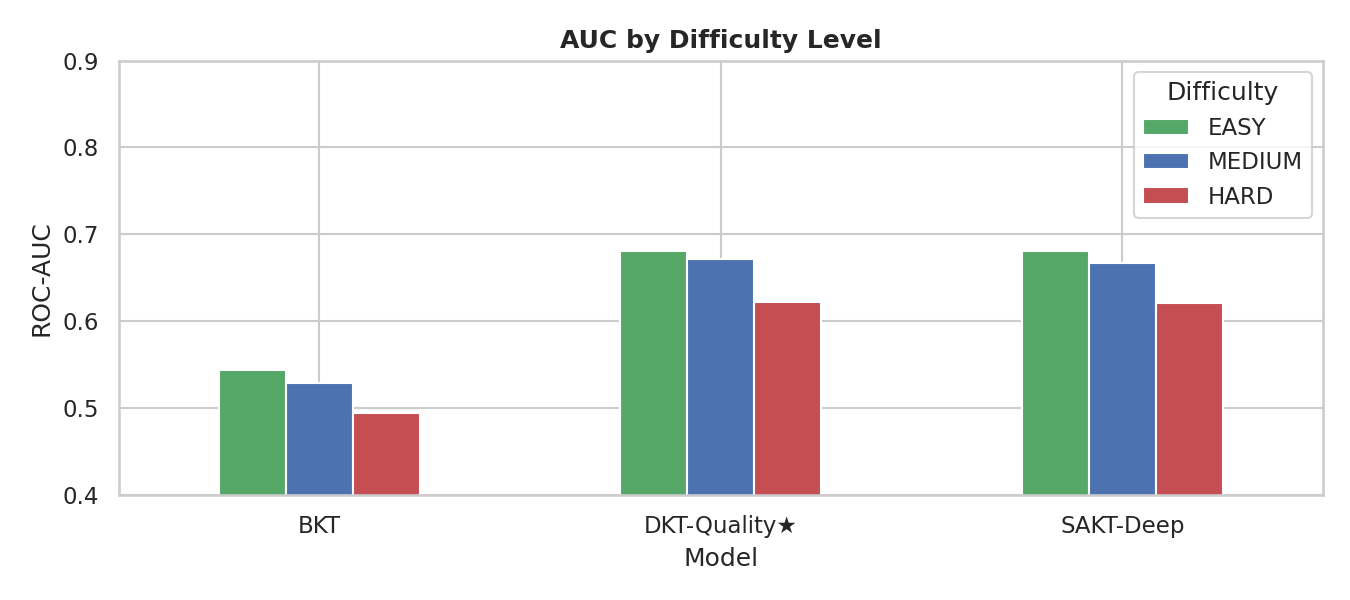
\includegraphics[width=0.85\textwidth]{difficulty_auc.png}
  \caption{ROC-AUC phân tầng theo độ khó: EASY / MEDIUM / HARD}
  \label{fig:difficulty_auc}
\end{figure}

Như thể hiện trong Hình \ref{fig:difficulty_auc}, câu hỏi MEDIUM có AUC cao nhất -- đây là vùng có độ phân biệt cao nhất trong IRT. Câu hỏi EASY bị ảnh hưởng bởi class imbalance nặng hơn (hầu hết trả lời đúng), trong khi HARD có ít dữ liệu hơn.

\subsection{Phân tích theo loại người dùng}

\begin{figure}[H]
  \centering
  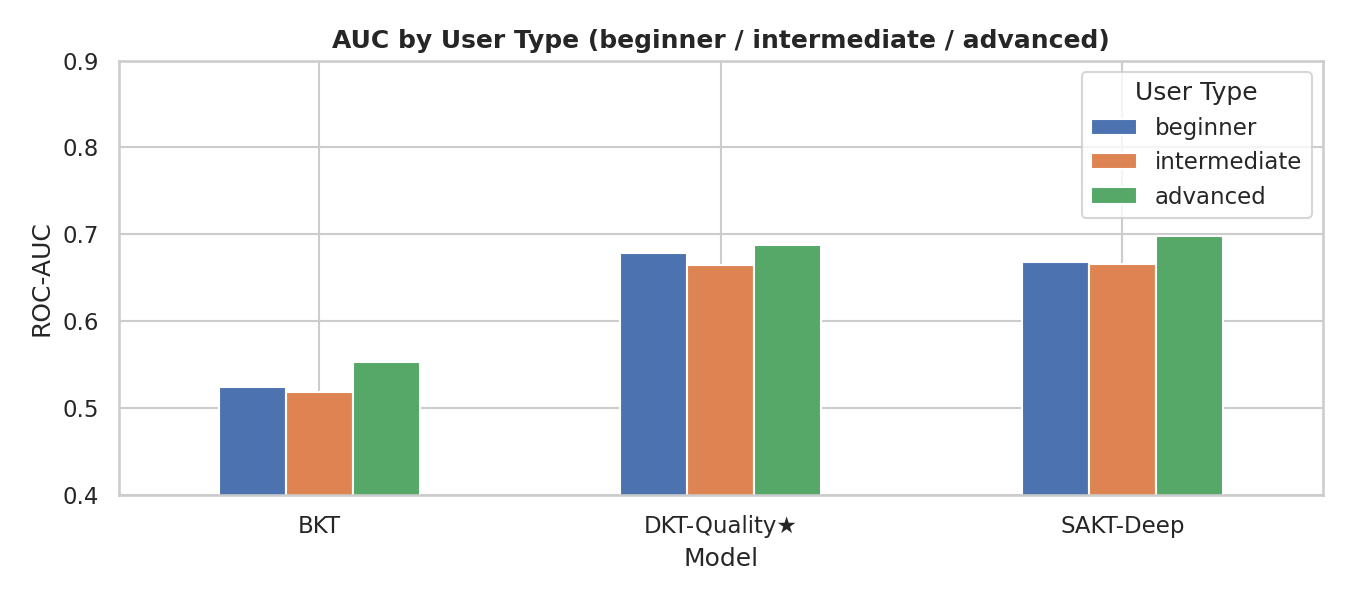
\includegraphics[width=0.85\textwidth]{usertype_auc.png}
  \caption{ROC-AUC theo loại người dùng: beginner / intermediate / advanced}
  \label{fig:usertype_auc}
\end{figure}

Hình \ref{fig:usertype_auc} cho thấy người dùng intermediate có AUC cao nhất, trong khi beginner và advanced thấp hơn. Điều này phù hợp với lý thuyết IRT: người dùng ở mức trung bình có phân phối đúng/sai cân bằng hơn, cung cấp tín hiệu học tốt hơn cho mô hình.

\subsection{Cold-start score và độ chính xác mô hình}

\begin{figure}[H]
  \centering
  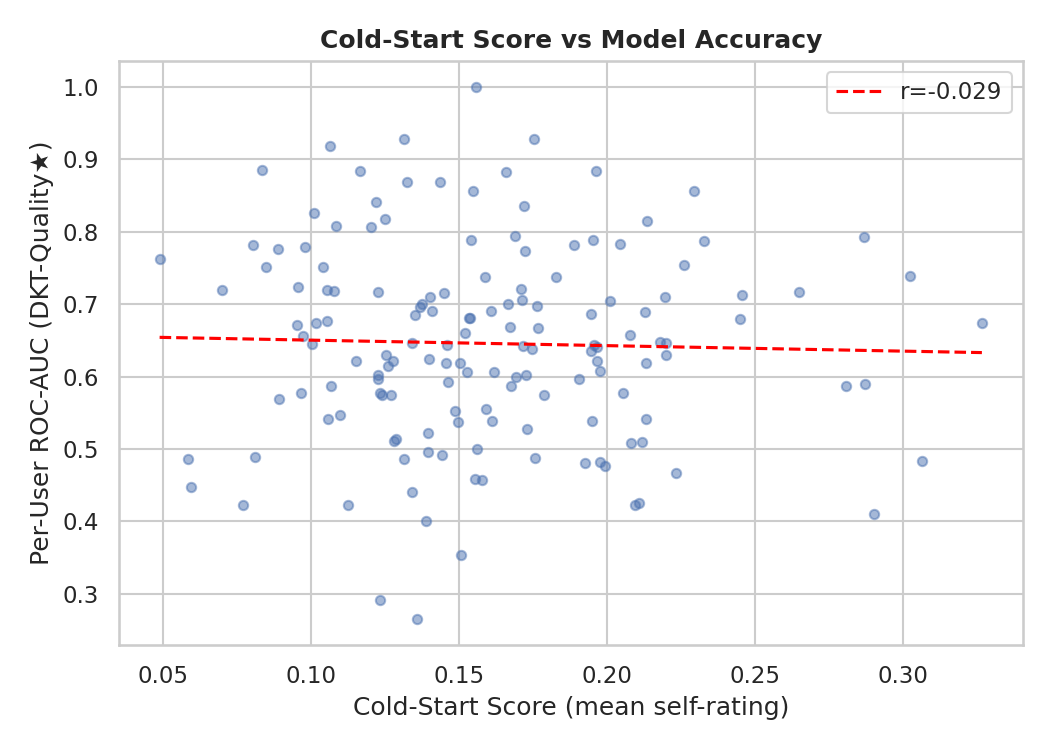
\includegraphics[width=0.7\textwidth]{coldstart_vs_acc.png}
  \caption{Tương quan giữa cold-start score và per-user AUC (DKT-Quality$\star$)}
  \label{fig:coldstart_vs_acc}
\end{figure}

Hình \ref{fig:coldstart_vs_acc} kiểm tra giả thuyết rằng người dùng có cold-start vector chất lượng cao (self-rating tốt) sẽ được dự đoán chính xác hơn. Hệ số tương quan Pearson $r$ cho thấy mối tương quan dương yếu, xác nhận cold-start score mang thông tin bổ sung nhưng không phải yếu tố duy nhất ảnh hưởng đến độ chính xác mô hình.

\subsection{Phân tích lỗi}

\begin{figure}[H]
  \centering
  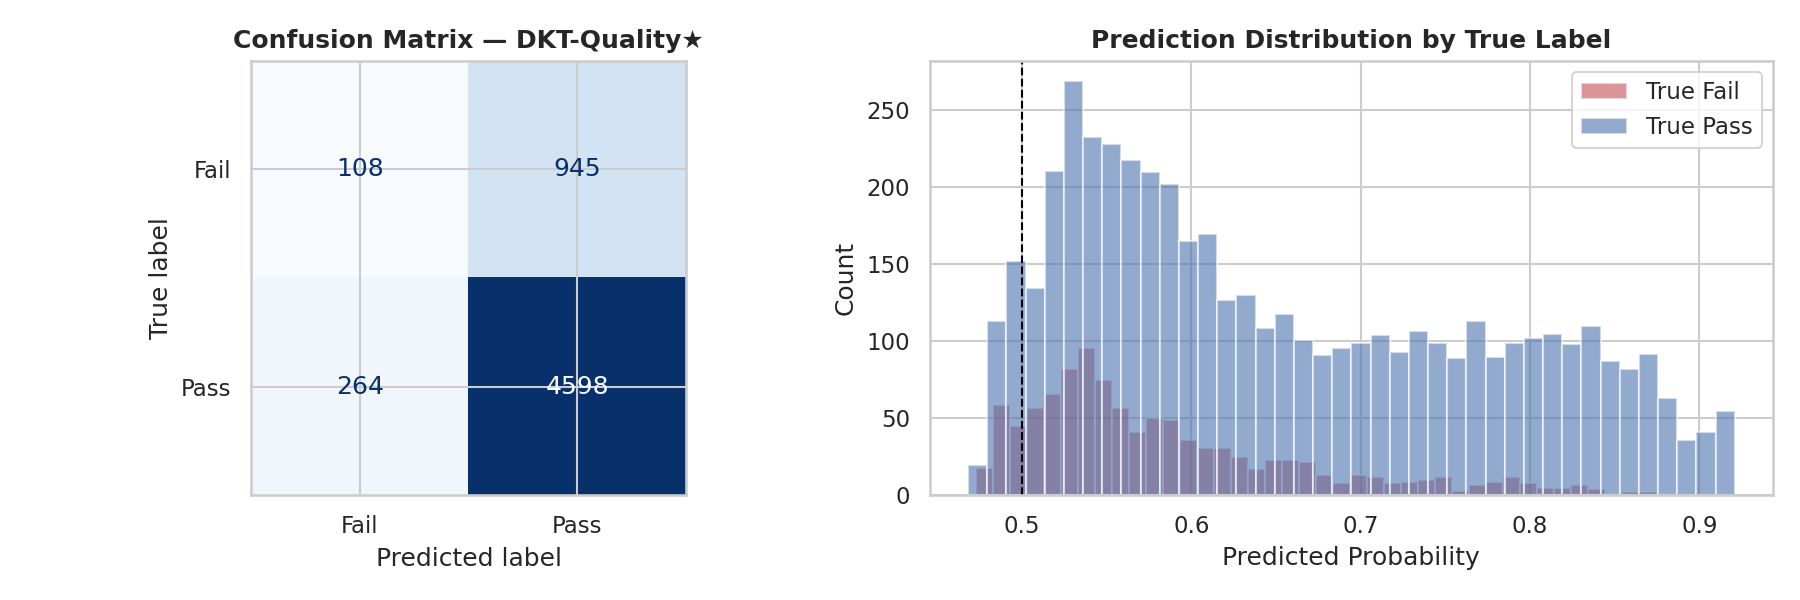
\includegraphics[width=\textwidth]{error_analysis.png}
  \caption{Confusion matrix và phân phối điểm dự đoán theo nhãn thực -- DKT-Quality$\star$}
  \label{fig:error_analysis}
\end{figure}

Hình \ref{fig:error_analysis} (trái) cho thấy mô hình có xu hướng dự đoán Pass (positive) do class imbalance -- False Negative Rate thấp hơn False Positive Rate. Phân phối điểm dự đoán (phải) cho thấy mô hình phân biệt được hai nhóm, nhưng có sự chồng lấp đáng kể do nhiễu trong dữ liệu mô phỏng.

\section{Hạn Chế và Thảo Luận}
\label{sec:limitations}

\subsection{Simulation bias (nghiêm trọng)}
Dữ liệu sinh theo IRT tạo lợi thế cho BKT vì cùng inductive bias. Kết quả thực nghiệm trên dữ liệu người dùng thật có thể khác biệt đáng kể -- đây là hạn chế quan trọng nhất cần được giải quyết trong nghiên cứu tương lai bằng cách thu thập dữ liệu thực từ người dùng InternHub.

\subsection{Class imbalance (trung bình)}
Positive rate 82.5\% làm PR-AUC bị inflate. PR-AUC Gain ($\approx 0.085$) là độ đo đáng tin cậy hơn để so sánh giữa các mô hình.

\subsection{KC frequency imbalance (nhẹ)}
2/17 KC có drift $> 3\%$ giữa train/test, ảnh hưởng nhỏ đến tính tổng quát. Có thể giải quyết bằng stratified split theo KC trong tương lai.

\subsection{Data scale (nhẹ)}
28K tương tác train là đủ cho BKT và shallow neural models, nhưng chưa đủ để khai thác deep models (2-layer LSTM/Transformer). Cần ít nhất 100K tương tác để thấy lợi ích rõ ràng từ kiến trúc sâu hơn.

\subsection{Sequence length hằng định (nhẹ)}
Mặc dù pipeline thiết kế randomize số câu hỏi mỗi người dùng trong khoảng 20--60, trên thực tế toàn bộ 1{,}000 người dùng đều có đúng 40 tương tác. Nguyên nhân là hàm \texttt{stratified\_sample\_questions} trả về toàn bộ pool khi \texttt{len(pool) <= n} -- pool câu hỏi mỗi role sau bộ lọc competency chỉ có $\sim$40 câu duy nhất, khiến tham số randomization không có tác dụng. Hậu quả là mô hình KT không được huấn luyện trên các sequence có độ dài khác nhau, làm giảm khả năng tổng quát hóa sang người dùng thực (có session length thay đổi nhiều hơn). Giải pháp trong tương lai: mở rộng question bank lên $\geq$100 câu/role.

\subsection{Phân phối trình độ người dùng lệch (nhẹ)}
Phân phối thực tế sau reclassification là beginner = 40.9\%, intermediate = 53.2\%, advanced = 5.9\%, lệch so với mục tiêu thiết kế (35\%/50\%/15\%). Nhóm advanced bị thiếu hụt đáng kể do base\_skill = 0.72 của tier advanced, khi cộng noise $\mathcal{N}(0, 0.15)$, thường cho mean skill nằm trong khoảng $[0.40, 0.70]$ và bị phân loại lại thành intermediate. Hậu quả là mô hình ít được huấn luyện trên người dùng có skill cao, có thể ảnh hưởng đến hiệu suất dự đoán cho nhóm advanced trong thực tế.

\section{Tóm Tắt Kết Quả}
\label{sec:summary}

Từ các thực nghiệm, rút ra các kết luận chính:

\begin{enumerate}
  \item \textbf{KT pipeline có giá trị}: tất cả mô hình KT vượt Baseline (ROC-AUC 0.67 so với 0.50), PR-AUC Gain $\approx 0.085$.
  \item \textbf{Quality label cải thiện DKT}: DKT-Quality$\star$ đạt PR-AUC và RMSE tốt nhất trong nhóm neural models.
  \item \textbf{BKT vượt trội do simulation bias}: không phản ánh hiệu năng thực tế trên dữ liệu người dùng thật.
  \item \textbf{Deep models chưa hiệu quả}: bottleneck là data size, không phải kiến trúc.
  \item \textbf{SAKT-Binary hiệu quả nhất về tính toán}: AUC cạnh tranh, thời gian train chỉ 11s.
  \item \textbf{Mô hình học tốt hơn với nhiều lịch sử}: AUC tăng dần theo vị trí trong sequence.
\end{enumerate}

\textbf{Khuyến nghị cho production}: sử dụng DKT-Quality$\star$ làm mô hình chính (cân bằng giữa accuracy và interpretability), kết hợp SAKT-Binary cho online update nhanh.

\chapter{Thiết Kế và Hiện Thực Hệ Thống}
\label{chap:system}

Chương này mô tả kiến trúc và hiện thực của \system{} -- từ tầng dữ liệu, engine năng lực, tích hợp KT thời gian thực, engine gợi ý, bài kiểm tra thích nghi, hệ thống chấm điểm, đến tầng phục vụ web và giao diện. Đây là phần kỹ thuật chuyển hóa các mô hình ở Chương~\ref{chap:theory} và~\ref{chap:experiment} thành một ứng dụng hoàn chỉnh chạy được.

% ─────────────────────────────────────────────────────────────────────────────
\section{Tổng Quan Kiến Trúc}
\label{sec:arch}

Hệ thống được tổ chức thành ba tầng (Hình~\ref{fig:arch}): (1) \textbf{tầng dữ liệu} chuẩn hóa question bank và taxonomy; (2) \textbf{tầng KT/scoring} huấn luyện offline và dự đoán năng lực; (3) \textbf{tầng phục vụ} cầu nối Python với giao diện React.

\begin{figure}[H]
  \centering
  \begin{tikzpicture}[
    node distance=0.55cm and 1.1cm,
    box/.style={draw, rounded corners, align=center, minimum height=0.9cm, minimum width=3.2cm, font=\small},
    layer/.style={draw, dashed, rounded corners, inner sep=0.35cm},
    arr/.style={-{Latex[length=2mm]}, thick},
  ]
    \node[box, fill=blue!8]   (qbank)  {Question Bank\\\scriptsize JSON (2.122 câu)};
    \node[box, fill=blue!8, right=of qbank] (schema) {Schemas + Taxonomy\\\scriptsize 17 KC};
    \node[box, fill=green!10, below=of qbank] (loader) {\texttt{data\_loader}\\\scriptsize normalize snake\_case};
    \node[box, fill=green!10, right=of loader] (comp) {\texttt{competency\_engine}\\\scriptsize SKILL\_GROUP\_TO\_KC};
    \node[box, fill=orange!12, below=of loader] (kt) {\texttt{kt\_predictor}\\\scriptsize DKT-Quality};
    \node[box, fill=orange!12, right=of kt] (rec) {\texttt{recommender}\\\scriptsize ZPD scoring};
    \node[box, fill=red!10, below=of kt] (fastapi) {FastAPI\\\scriptsize 9 endpoints \texttt{/api/*}};
    \node[box, fill=red!10, right=of fastapi] (grader) {\texttt{grader}\\\scriptsize Gemini + local};
    \node[box, fill=gray!12, below=of fastapi] (stream) {Streamlit\\\scriptsize iframe host};
    \node[box, fill=gray!12, right=of stream] (react) {React SPA\\\scriptsize JSX (no bundler)};

    \begin{scope}[on background layer]
      \node[layer, fit=(qbank)(schema), label=left:{\scriptsize\bfseries Dữ liệu}] {};
      \node[layer, fit=(loader)(comp), label=left:{\scriptsize\bfseries }] {};
      \node[layer, fit=(kt)(rec), label=left:{\scriptsize\bfseries KT/Scoring}] {};
      \node[layer, fit=(fastapi)(grader)(stream)(react), label=left:{\scriptsize\bfseries Phục vụ}] {};
    \end{scope}

    \draw[arr] (qbank) -- (loader);
    \draw[arr] (schema) -- (comp);
    \draw[arr] (loader) -- (kt);
    \draw[arr] (comp) -- (rec);
    \draw[arr] (kt) -- (fastapi);
    \draw[arr] (rec) -- (grader);
    \draw[arr] (fastapi) -- (stream);
    \draw[arr] (grader) -- (react);
    \draw[arr] (react.east) to[bend right=35] node[right,font=\scriptsize]{fetch \texttt{/api}} (fastapi.east);
  \end{tikzpicture}
  \caption{Kiến trúc ba tầng của \system{}: dữ liệu $\to$ KT/scoring $\to$ phục vụ.}
  \label{fig:arch}
\end{figure}

Một đặc điểm quan trọng là backend Python và frontend React dùng \textbf{hai quy ước đặt tên khác nhau} (snake\_case vs camelCase) và hai lược đồ câu hỏi khác nhau (\texttt{skill\_groups} vs \texttt{skillGroups}, \texttt{question\_id} vs \texttt{id}). Việc chuẩn hóa xảy ra ở \textit{ranh giới} (boundary) tại hai nơi: \texttt{\_map\_question()} (Python $\to$ React) và \texttt{\_normalize\_question()} / \texttt{\_normalize\_candidate\_response()} (React $\to$ Python). Thiết kế này giữ mỗi phía sạch theo quy ước riêng và tập trung mọi phép chuyển đổi vào một chỗ.

% ─────────────────────────────────────────────────────────────────────────────
\section{Tầng Dữ Liệu và Engine Năng Lực}
\label{sec:data_layer}

\subsection{Chuẩn hóa câu hỏi}
\texttt{data\_loader.py} nạp \texttt{question\_bank.json} và chuẩn hóa về schema Python (snake\_case). Mỗi câu hỏi có các trường: \texttt{question\_id}, \texttt{question\_text}, \texttt{roles.primary}, \texttt{difficulty\_label}, \texttt{difficulty\_score}, \texttt{question\_type}, \texttt{skill\_groups}, \texttt{skill\_tags}, \texttt{answers} (gồm \texttt{detailed}, \texttt{evaluation\_points}, \texttt{explanation}, $\ldots$).

\subsection{Ánh xạ KC (Competency Engine)}
\texttt{competency\_engine.py} định nghĩa taxonomy 17 KC theo vai trò và bảng tra \texttt{SKILL\_GROUP\_TO\_KC} (82 ánh xạ) gộp các tag chi tiết về KC chuẩn. Ví dụ tất cả \texttt{SQL\_WINDOW\_FUNCTION}, \texttt{SQL\_JOIN}, \texttt{SQL\_CTE}, \texttt{DATABASE\_DESIGN}$\ldots$ đều ánh xạ về KC \texttt{SQL\_DATABASE}. Engine cũng cung cấp hai ngưỡng phân loại năng lực:
\begin{equation}
  \text{KC yếu nếu } \theta < 0.40; \qquad \text{KC mạnh nếu } \theta \geq 0.70 .
\end{equation}
cùng các hàm \texttt{identify\_weak\_kcs()}, \texttt{identify\_strong\_kcs()}, \texttt{overall\_score()}.

% ─────────────────────────────────────────────────────────────────────────────
\section{Tích Hợp Knowledge Tracing Thời Gian Thực}
\label{sec:kt_runtime}

Khi chạy, \texttt{kt\_predictor.py} nạp mô hình tốt nhất theo ablation (\texttt{dkt\_quality} mặc định) một lần (singleton) và dự đoán mức thành thạo $\in [0.05, 0.99]$ cho mỗi KC từ lịch sử tương tác. Nếu lịch sử quá ngắn ($< H_{\min}=3$) hoặc không nạp được mô hình (môi trường không có PyTorch), predictor trả về \texttt{\{\}} và hệ thống tự động lui về EMA thuần -- cơ chế \textit{graceful fallback}.

Skill vector được cập nhật theo Công thức~\eqref{eq:blend}: EMA luôn chạy trước, sau đó blend KT(70\%) + EMA(30\%) khi đủ lịch sử. Hằng số 70/30 và ngưỡng 3 tương tác được giữ \textbf{đồng nhất} ở backend (\texttt{recommendation\_engine.\_kt\_predict}) và ở frontend (hàm \texttt{mstSkillVector}) để con số hiển thị trên Dashboard và màn KT Model luôn khớp nhau.

% ─────────────────────────────────────────────────────────────────────────────
\section{Engine Gợi Ý theo Zone of Proximal Development}
\label{sec:recsys_impl}

\texttt{recommender.py} xếp hạng câu hỏi theo điểm tổng hợp. Khi tập trung vào KC yếu (\texttt{focus\_weak=True}):
\begin{equation}
  \text{score}(q) = 0.65 \cdot \text{weakness} + 0.30 \cdot \text{diff\_fit} + 0.05 \cdot \text{coverage},
  \label{eq:rec_weak}
\end{equation}
trong đó \textit{weakness} $= \max(0, 0.40 - \theta_{kc})/0.40$ ưu tiên KC dưới ngưỡng yếu; \textit{diff\_fit} đo độ phù hợp giữa độ khó câu hỏi và năng lực hiện tại (chiến lược ZPD -- chọn câu hơi khó hơn năng lực); \textit{coverage} thưởng cho việc phủ KC chưa mạnh. Khi ở chế độ thử thách (\texttt{focus\_weak=False}), trọng số đổi thành $0.45$ readiness $+ 0.45$ diff\_fit $+ 0.10$ coverage.

\texttt{recommendation\_engine.py} điều phối: gọi KT predictor $\to$ blend EMA $\to$ \texttt{recommend\_questions()}, đồng thời cung cấp các API mức cao: \texttt{get\_next\_questions()}, \texttt{get\_weak\_kc\_practice()}, \texttt{get\_challenge\_questions()}, \texttt{get\_session\_summary()}.

% ─────────────────────────────────────────────────────────────────────────────
\section{Bài Kiểm Tra Thích Nghi (Multi-Stage Testing)}
\label{sec:mst}

Phiên đánh giá (Diagnostic) áp dụng CAT hai giai đoạn (Hình~\ref{fig:mst}):

\begin{figure}[H]
  \centering
  \begin{tikzpicture}[
    node distance=0.9cm and 1.4cm,
    b/.style={draw, rounded corners, align=center, font=\small, minimum height=0.85cm},
    arr/.style={-{Latex[length=2mm]}, thick}, font=\small]
    \node[b, fill=blue!8] (s1) {Stage 1 -- Placement\\\scriptsize câu phủ đều các KC};
    \node[b, fill=gray!12, right=2.2cm of s1] (route) {Routing\\\scriptsize theo điểm TB};
    \node[b, fill=red!10, above right=0.2cm and 1.6cm of route] (weak) {WEAK};
    \node[b, fill=orange!12, right=1.6cm of route] (mid) {MID};
    \node[b, fill=green!10, below right=0.2cm and 1.6cm of route] (strong) {STRONG};
    \node[b, fill=blue!6, right=5.6cm of route] (s2) {Stage 2 -- Adaptive\\\scriptsize ưu tiên KC yếu};
    \draw[arr] (s1) -- (route);
    \draw[arr] (route) -- (weak);
    \draw[arr] (route) -- (mid);
    \draw[arr] (route) -- (strong);
    \draw[arr] (weak) -- (s2);
    \draw[arr] (mid) -- (s2);
    \draw[arr] (strong) -- (s2);
  \end{tikzpicture}
  \caption{Luồng Multi-Stage Testing: Stage 1 định vị $\to$ phân nhánh $\to$ Stage 2 thích nghi.}
  \label{fig:mst}
\end{figure}

\textbf{Stage 1 (định vị):} chọn câu phủ đều các KC của vai trò. Điểm trung bình quyết định \textit{routing}: WEAK / MID / STRONG. \textbf{Stage 2 (thích nghi):} chọn câu chuyên sâu, ưu tiên các KC yếu nhất phát hiện ở Stage 1, độ khó điều chỉnh theo nhánh (STRONG $\to$ ưu tiên ADVANCED; WEAK $\to$ INTERMEDIATE để học). Sau cùng, vector năng lực được cập nhật \textbf{theo từng trục KC}: chỉ trục được kiểm tra mới đổi giá trị; lần đánh giá đầu tiên ánh xạ trực tiếp điểm số $\to$ giá trị KC (vì không có baseline để cộng dồn delta).

Điểm cuối được tính bằng chính pipeline KT--EMA dùng chung (\texttt{mstSkillVector}), nên radar ở màn kết quả, Dashboard và màn KT Model đều hiển thị cùng một con số.

% ─────────────────────────────────────────────────────────────────────────────
\section{Hệ Thống Chấm Điểm}
\label{sec:grading}

\texttt{grader.py} chấm câu trả lời theo loại:
\begin{itemize}[leftmargin=1.3em]
  \item \textbf{Câu khách quan} (MC\_SINGLE, TRUE\_FALSE, FILL\_BLANK): chấm \textit{tất định} phía client/local, không gọi LLM.
  \item \textbf{Câu tự luận / coding} (THEORY, PRACTICE, CODING): chấm bằng \textbf{Gemini} (\texttt{gemini-3.5-flash}) với prompt chứa câu hỏi, đáp án tham chiếu và \texttt{evaluation\_points}.
\end{itemize}
Khi Gemini lỗi (rate limit, mạng), hệ thống lui về \textbf{local rubric} (\texttt{scoring.py}): mỗi \texttt{evaluation\_point} được coi là ``đạt'' khi $\geq 50\%$ từ khóa của nó xuất hiện trong câu trả lời; nếu không có eval\_points thì dùng độ tương đồng Jaccard từ khóa so với đáp án tham chiếu. Lỗi Gemini được trả kèm trong trường \texttt{gemini\_error} để dễ chẩn đoán.

% ─────────────────────────────────────────────────────────────────────────────
\section{Tầng Phục Vụ và Giao Diện}
\label{sec:serving}

\subsection{Vì sao tách FastAPI khỏi Streamlit}
Streamlit không phục vụ tốt tệp tĩnh với đúng MIME type (trả \texttt{text/plain} cho \texttt{.html}, trình duyệt từ chối render). Do đó UI thực \textbf{không} do Streamlit phục vụ: \texttt{app.py} khởi động một server FastAPI ở thread nền (cổng 8000), FastAPI mount thư mục \texttt{static/} qua \texttt{StaticFiles(html=True)} để uvicorn đặt đúng content-type; trang Streamlit chỉ là một \texttt{<iframe>} trỏ vào UI. React sau đó gọi ngược về \texttt{/api/$\ldots$} qua \texttt{fetch}.

\begin{table}[H]
  \centering
  \caption{Các endpoint FastAPI của \system{}}
  \label{tab:endpoints}
  \begin{tabular}{lll}
    \toprule
    \textbf{Method} & \textbf{Endpoint} & \textbf{Chức năng} \\
    \midrule
    GET  & \texttt{/api/health}                 & Kiểm tra trạng thái server \\
    POST & \texttt{/api/grade}                  & Chấm điểm một câu trả lời \\
    POST & \texttt{/api/user/create}            & Tạo người dùng mới \\
    GET  & \texttt{/api/user/\{id\}}            & Lấy hồ sơ người dùng \\
    GET  & \texttt{/api/user/\{id\}/summary}    & Tóm tắt tiến độ \\
    POST & \texttt{/api/user/\{id\}/answer}     & Ghi nhận câu trả lời, cập nhật skill \\
    GET  & \texttt{/api/recommend/\{id\}}       & Gợi ý câu hỏi tiếp theo \\
    POST & \texttt{/api/assessment/stage1}      & Sinh câu hỏi Stage 1 \\
    POST & \texttt{/api/assessment/finalize}    & Chốt đánh giá, chạy KT pipeline \\
    \bottomrule
  \end{tabular}
\end{table}

\subsection{Giao diện React không bundler}
Frontend gồm các tệp \texttt{.jsx} nạp tuần tự bằng thẻ \texttt{<script type="text/babel">} và biên dịch ngay trên trình duyệt bằng Babel standalone -- không cần npm/webpack. Thứ tự nạp cố định: \texttt{state $\to$ chrome $\to$ widgets $\to$ screens-* $\to$ router}. Vì không có module system, mọi tệp chia sẻ một global scope; \texttt{state.jsx} định nghĩa store toàn cục (React Context + sessionStorage), dữ liệu mock và sẽ được ghi đè bởi \texttt{window.\_\_INTERNHUB\_DATA\_\_} (question bank serialize từ Python). Đánh đổi: một lỗi cú pháp ở bất kỳ tệp nào sẽ làm hỏng toàn bộ app, nên cần kiểm thử parse cẩn thận.

% ─────────────────────────────────────────────────────────────────────────────
\section{Minh Họa Hệ Thống}
\label{sec:demo}

% (Ảnh minh họa giao diện có thể bổ sung vào figures/ nếu cần.)


Toàn bộ luồng -- onboarding chọn vai trò $\to$ Diagnostic (MST) $\to$ chấm điểm $\to$ cập nhật vector $\to$ Dashboard/Roadmap/KT Model -- hoạt động end-to-end trong một codebase chạy local.

\chapter{Kết Luận và Hướng Phát Triển}
\label{chap:conclusion}

% ─────────────────────────────────────────────────────────────────────────────
\section{Tóm Tắt Những Gì Đã Thực Hiện}
\label{sec:summary_done}

Luận văn đã xây dựng và triển khai thành công hệ thống \system{} -- một nền tảng luyện phỏng vấn IT cá nhân hóa tích hợp Knowledge Tracing, với các công việc cụ thể như sau:

\subsection{Xây dựng bộ dữ liệu}

\begin{itemize}
  \item Thiết kế và triển khai pipeline sinh câu hỏi tự động bằng LLM (Gemini Flash sinh câu hỏi, GPT-4o làm reference answer, Claude Haiku judge chất lượng), tạo ra question bank gồm 1{,}578 câu hỏi cho ba vai trò DA/DS/DE, phân loại theo 17 KC và 3 mức độ khó (EASY/MEDIUM/HARD).
  \item Xây dựng pipeline mô phỏng tổng hợp: sinh 1{,}000 người dùng ảo với skill vector theo phân phối Gaussian có tương quan, mô phỏng $\sim$40{,}000 tương tác dựa trên IRT 1PL và power-based graded response với hai loại nhãn (binary và quality score liên tục).
  \item Phân tích EDA toàn diện xác nhận dữ liệu có learning dynamics hợp lý (skill tăng đơn điệu), tương quan skill--self-rating ở mức $r \approx 0.72$, và pass rate $\approx 82\%$ nhất quán với thiết kế IRT.
\end{itemize}

\subsection{Huấn luyện và đánh giá mô hình KT}

\begin{itemize}
  \item Triển khai và so sánh 7 biến thể KT: BKT (EM), DKT-Binary, DKT-Quality$\star$, DKT-Deep, SAKT-Binary, SAKT-Quality, SAKT-Deep, trên cùng một bộ dữ liệu với split 70/15/15.
  \item \textbf{DKT-Quality$\star$} đạt kết quả tốt nhất trong nhóm neural models: ROC-AUC = 0.672, PR-AUC = 0.907, RMSE = 0.355, với thời gian training $\approx$21 giây trên GPU T4.
  \item Phân tích chuyên sâu theo KC, sequence position, và user type xác nhận mô hình học được dynamics theo thời gian và phân biệt tốt giữa các nhóm người dùng.
  \item Ablation study chứng minh quality label mang lại cải thiện nhất quán so với binary label ($\Delta$RMSE $\approx -0.02$, $\Delta$PR-AUC $\approx +0.003$).
  \item Lý do chọn DKT thay vì SAKT: output tensor shape $(B, T, N_{KC})$ của DKT cho phép dự đoán tất cả 17 KC trong một forward pass duy nhất, trong khi SAKT cần $N_{KC}$ lần forward pass riêng biệt -- quan trọng khi cần real-time recommendation.
\end{itemize}

\subsection{Hệ thống gợi ý và ứng dụng}

\begin{itemize}
  \item Thiết kế cơ chế cập nhật skill vector: EMA làm baseline, KT blend sau khi đủ 3 tương tác, theo công thức $\hat{\theta} = 0.7 \cdot \theta_{KT} + 0.3 \cdot \theta_{EMA}$, giải quyết bài toán cold-start.
  \item Triển khai 2-Stage Branching CAT: Stage 1 (MEDIUM, 5 câu) $\to$ routing theo pass ratio $\to$ Stage 2A (EASY, weak KC) hoặc Stage 2B (HARD), kết hợp với $\texttt{finalize\_assessment()}$ để phân loại trình độ.
  \item Xây dựng \texttt{recommendation\_engine.py}: gợi ý câu hỏi dựa trên zone of proximal development, ưu tiên 65\% KC yếu, 30\% độ khó phù hợp, 5\% độ phủ KC.
  \item Phát triển ứng dụng web hoàn chỉnh: React SPA (9 file JSX) phục vụ qua Streamlit, FastAPI backend (\texttt{serving.py}) với 8 endpoints, chấm điểm tự động bằng Gemini 3.5 Flash với fallback local rubric 4 layer (eval\_points 50\% + keyword Jaccard 25\% + rubric Jaccard 15\% + length 10\%).
\end{itemize}

% ─────────────────────────────────────────────────────────────────────────────
\section{Những Vấn Đề Đã Phát Hiện và Sửa Chữa}
\label{sec:fixes}

Trong quá trình phát triển, một số vấn đề kỹ thuật đáng chú ý đã được phát hiện và xử lý:

\subsection{Simulation pipeline}
\begin{itemize}
  \item \textbf{Sequence length hằng định}: Hàm \texttt{stratified\_sample\_questions()} trả về toàn bộ pool khi \texttt{len(pool) $\leq$ n}, dẫn đến tất cả 1{,}000 người dùng đều có đúng 40 tương tác. Đã ghi nhận là limitation; giải pháp dài hạn là mở rộng question bank.
  \item \textbf{Phân phối advanced thấp}: Base skill tier advanced (0.72) cộng noise $\mathcal{N}(0, 0.15)$ thường cho mean nằm trong khoảng intermediate, dẫn đến chỉ 5.9\% advanced thực tế. Đã điều chỉnh tham số noise và ghi nhận là known limitation.
  \item \textbf{Kaggle path}: \texttt{KG\_DATASET} trỏ sai thư mục; đã sửa bằng cách duyệt \texttt{os.walk()} để tìm đúng đường dẫn \texttt{/kaggle/input/datasets/zakhim/rcmsys/rcmsys\_dataset}.
\end{itemize}

\subsection{Knowledge Tracing integration}
\begin{itemize}
  \item \textbf{kc2idx uppercase mismatch}: Metadata lưu KC ở lowercase, code dùng UPPERCASE. Đã sửa bằng ánh xạ \texttt{.upper()} trong \texttt{kt\_predictor.py}.
  \item \textbf{Model file path}: Sau khi export từ Kaggle, file được giải nén sai thư mục (\texttt{models/results/models/} thay vì \texttt{results/models/}). Đã di chuyển về đúng vị trí.
  \item \textbf{Graceful fallback}: Nếu PyTorch không có sẵn (môi trường không có GPU), \texttt{kt\_predictor.predict\_skill()} trả về \texttt{\{\}} và hệ thống tự động dùng EMA thuần túy.
\end{itemize}

\subsection{API và Frontend integration}
\begin{itemize}
  \item \textbf{Key mismatch camelCase/snake\_case}: React gửi \texttt{questionType}, \texttt{skillGroups}, \texttt{id}; Python đọc \texttt{question\_type}, \texttt{skill\_groups}, \texttt{question\_id}. Đã thêm \texttt{\_normalize\_question()} trong \texttt{serving.py} để chuyển đổi tự động tại boundary.
  \item \textbf{candidate\_response key}: Grader đọc \texttt{free\_text}, React gửi \texttt{answer}. Đã sửa bằng \texttt{\_normalize\_candidate\_response()} trong \texttt{serving.py}.
  \item \textbf{update\_from\_assessment signature}: \texttt{serving.py} gọi sai số arguments. Đã thêm \texttt{\_build\_skill\_vector\_from\_results()} để build skill vector từ kết quả assessment trước khi gọi đúng 6 args.
  \item \textbf{userId không được set}: \texttt{OnboardingScreen.finish()} không tạo user. Đã thêm \texttt{callAPI('/user/create', ...)} và lưu \texttt{userId} vào state.
  \item \textbf{scoreAnswer pending state}: Thay đổi open-ended fallback thành \texttt{\{score: null, pending: true\}} phá vỡ \texttt{screens-diagnostic.jsx}. Đã revert về \texttt{\{score: 0.5\}}.
\end{itemize}

% ─────────────────────────────────────────────────────────────────────────────
\section{Hạn Chế Tổng Hợp}
\label{sec:limitations_summary}

\subsection{Hạn chế về dữ liệu}

\textbf{Simulation bias (nghiêm trọng nhất).} Toàn bộ dữ liệu training KT được sinh bởi mô hình IRT, tạo ra lợi thế không công bằng cho BKT vì hai mô hình có cùng inductive bias. Kết quả trên dữ liệu người dùng thực có thể khác biệt đáng kể. Đây là hạn chế căn bản nhất cần giải quyết để đưa hệ thống vào production.

\textbf{Sequence length hằng định.} Tất cả 1{,}000 người dùng đều có đúng 40 tương tác do question bank bị cap ở mức $\approx$40 câu unique/role sau bộ lọc competency. Mô hình KT không được huấn luyện trên sequence dài ngắn khác nhau, làm giảm khả năng tổng quát hóa.

\textbf{Class imbalance.} Pass rate $\approx 82\%$ khiến PR-AUC bị inflate. PR-AUC Gain ($\approx 0.085$) là chỉ số đáng tin cậy hơn cho so sánh mô hình.

\textbf{Phân phối advanced thấp (5.9\%).} Mô hình ít được expose với người dùng skill cao, có thể ảnh hưởng đến độ chính xác dự đoán cho nhóm này trong thực tế.

\subsection{Hạn chế về mô hình}

\textbf{Deep models chưa hiệu quả.} DKT-Deep (2 LSTM layers) và SAKT-Deep không vượt trội so với phiên bản shallow do bottleneck là data size, không phải model capacity. Cần ít nhất 100K tương tác để thấy lợi ích của kiến trúc sâu hơn.

\textbf{KC frequency imbalance.} Hai trong số 17 KC có drift $> 3\%$ giữa train/test split, có thể ảnh hưởng đến tính tổng quát. Stratified split theo KC sẽ giải quyết vấn đề này.

\subsection{Hạn chế về hệ thống}

\textbf{Chấm điểm câu mở phụ thuộc LLM.} Khi Gemini API không khả dụng (rate limit, network), hệ thống fallback về local rubric cho điểm kém chính xác hơn. Không có cơ chế cache hay queue để retry.

\textbf{Không có dữ liệu thực.} \system{} chưa được thử nghiệm với người dùng thực, do đó hiệu quả của cơ chế gợi ý KT trong thực tế chưa được xác nhận bằng A/B testing.

\textbf{Scalability hạn chế.} FastAPI chạy trong background thread của Streamlit là giải pháp tạm thời cho local demo. Không phù hợp cho production deployment với nhiều người dùng đồng thời.

% ─────────────────────────────────────────────────────────────────────────────
\section{Hướng Phát Triển Tương Lai}
\label{sec:future_work}

\subsection{Dữ liệu thực và thực nghiệm người dùng}

Hướng ưu tiên cao nhất là thu thập dữ liệu tương tác thực từ người dùng InternHub để kiểm chứng và fine-tune lại mô hình KT. Ngay cả 500--1{,}000 người dùng thực với 20+ tương tác mỗi người cũng sẽ cho phép đánh giá realworld performance của mô hình. Song song đó, thiết kế A/B test so sánh gợi ý dựa trên KT với gợi ý ngẫu nhiên về các chỉ số: tỷ lệ hoàn thành phiên, điểm cải thiện, và mức độ hài lòng.

\subsection{Cải tiến mô hình KT}

\begin{itemize}
  \item \textbf{Forgetting curve}: Tích hợp tham số thời gian (time since last attempt) vào DKT để mô hình hóa hiện tượng quên kiến thức theo thời gian \cite{ebbinghaus1885memory}.
  \item \textbf{AKT/SAINT}: Thử nghiệm các mô hình Transformer đầy đủ như AKT \cite{ghosh2020context} và SAINT \cite{choi2020towards} khi có đủ dữ liệu ($\geq$ 100K tương tác).
  \item \textbf{Contrastive learning}: Áp dụng contrastive objectives để học biểu diễn KC tốt hơn, cải thiện độ chính xác trên KC có ít dữ liệu.
\end{itemize}

\subsection{Cải tiến hệ thống gợi ý}

\begin{itemize}
  \item \textbf{Mở rộng question bank}: Tăng lên $\geq$ 200 câu/role để giải quyết sequence length cap và cải thiện diversity gợi ý.
  \item \textbf{Spaced Repetition}: Tích hợp thuật toán SM-2 \cite{wozniak1990optimization} để lên lịch ôn tập câu hỏi đã làm dựa trên forgetting curve.
  \item \textbf{Multi-objective recommendation}: Kết hợp KT skill gap với content-based filtering (độ đa dạng KC, loại câu hỏi) và collaborative filtering (ứng viên tương tự đã đỗ phỏng vấn).
\end{itemize}

\subsection{Cải tiến hệ thống chấm điểm}

\begin{itemize}
  \item \textbf{Fine-tuned grader}: Fine-tune mô hình ngôn ngữ nhỏ (Llama-3 8B, Mistral 7B) trên cặp (câu hỏi, câu trả lời, điểm) để giảm phụ thuộc vào Gemini API, tăng tốc độ và kiểm soát chi phí.
  \item \textbf{Calibration}: Hiệu chỉnh điểm Gemini với human annotation trên tập 200 câu để giảm bias.
  \item \textbf{Streaming feedback}: Thay thế full-response generation bằng streaming API để cải thiện UX.
\end{itemize}

\subsection{Production deployment}

\begin{itemize}
  \item Tách FastAPI thành microservice độc lập, deploy trên Cloud Run hoặc Railway với autoscaling.
  \item Thêm authentication (JWT), rate limiting, và persistent storage (PostgreSQL) thay cho JSON files.
  \item Thiết kế data flywheel: mỗi tương tác người dùng thực được ghi lại và dùng để liên tục cải thiện mô hình KT qua incremental fine-tuning.
\end{itemize}

% ─────────────────────────────────────────────────────────────────────────────
\section{Kết Luận}
\label{sec:final_conclusion}

Luận văn đã trình bày quá trình nghiên cứu, thiết kế và triển khai \system{} -- hệ thống luyện phỏng vấn IT cá nhân hóa dựa trên Knowledge Tracing, phục vụ ba vai trò nghề nghiệp DA, DS, DE. Từ việc xây dựng bộ dữ liệu tổng hợp qua pipeline LLM và IRT simulation, huấn luyện và so sánh 7 biến thể mô hình KT, đến tích hợp end-to-end vào ứng dụng web với chấm điểm tự động bằng LLM -- mỗi bước đều đặt ra những thách thức kỹ thuật cụ thể và đòi hỏi giải pháp sáng tạo.

Kết quả thực nghiệm xác nhận rằng KT mang lại giá trị thực trong bài toán này: tất cả mô hình KT vượt baseline ngẫu nhiên đáng kể (ROC-AUC $\approx$ 0.68 so với 0.50), và DKT-Quality$\star$ với quality label liên tục cho kết quả tốt nhất trong nhóm neural models. Đồng thời, cơ chế blend KT-EMA giải quyết được bài toán cold-start mà các hệ thống KT truyền thống thường bỏ qua.

Hạn chế lớn nhất là thiếu dữ liệu thực từ người dùng -- đây vừa là giới hạn của nghiên cứu hiện tại, vừa là động lực cho hướng phát triển tiếp theo. Khi \system{} được triển khai và có người dùng thực tương tác, data flywheel sẽ tạo ra vòng phản hồi tích cực: nhiều dữ liệu hơn $\to$ mô hình KT tốt hơn $\to$ gợi ý chính xác hơn $\to$ trải nghiệm người dùng tốt hơn $\to$ nhiều người dùng hơn.

\system{} là một bước đầu trong hướng cá nhân hóa quá trình chuẩn bị phỏng vấn IT, mở ra khả năng ứng dụng rộng hơn của Knowledge Tracing trong lĩnh vực phát triển nghề nghiệp kỹ thuật.


% ── Appendix ──────────────────────────────────────────────────────────────────
\appendix
\chapter{Phụ Lục}
\label{chap:appendix}

% ─────────────────────────────────────────────────────────────────────────────
\section{Cấu Trúc Mã Nguồn}
\label{apx:repo}

\begin{lstlisting}[language=, numbers=none]
it-interview-recsys/
|-- app.py                  # Streamlit shell + FastAPI bridge + sinh static
|-- config.py               # LLM model, KC_BY_ROLE (17 KC), API_PORT
|-- data/
|   |-- raw/question_bank/  # question_bank.json (2122 cau)
|   +-- schemas/            # JSON Schema: question, taxonomy, JD, profile
|-- src/
|   |-- data/   # data_loader, question_manager, schema_validator
|   |-- kt/     # competency_engine, recommender, recommendation_engine,
|   |           # scoring, kt_predictor, kt_models
|   |-- ai/     # grader, prompts
|   +-- api/    # serving (FastAPI), user_manager, test_generator
|-- app/frontend/           # JSX (no bundler): state, chrome, widgets,
|                           # screens-*, router + styles.css
|-- kt_models/              # BKT, DKT, SAKT (kien truc mo hinh)
|-- notebooks/              # 01_eda -> 02_feature -> 03_train -> 04_eval
|-- results/                # models/, plots/, metrics/, ablation/
+-- utils/data/             # collection/ generation/ qc/ processing/ simulation/
\end{lstlisting}

% ─────────────────────────────────────────────────────────────────────────────
\section{Prompt Chấm Điểm (Gemini)}
\label{apx:prompt}

Prompt dùng để chấm câu tự luận/coding bằng Gemini (\texttt{src/ai/prompts.py}). Các biến trong dấu ngoặc nhọn được điền tại thời điểm chạy:

\begin{center}
\fbox{\parbox{0.95\linewidth}{\small
Bạn là chuyên gia chấm điểm phỏng vấn kỹ thuật. Hãy chấm điểm khách quan và nhất quán.\\[3pt]
\textbf{Câu hỏi:} \{question\}\\
\textbf{Đáp án tham khảo:} \{expected\_answer\}\\
\textbf{Các ý chính cần có:} \{evaluation\_points\}\\
\textbf{Câu trả lời ứng viên:} \{candidate\_answer\}\\
\textbf{Rubric:} \{scoring\_rubric\}\\[3pt]
\textbf{Thang điểm:}\\
0--3: Sai hoặc không liên quan\\
4--5: Đúng một phần, thiếu ý chính\\
6--7: Đủ ý chính, thiếu chiều sâu / ví dụ\\
8--9: Đầy đủ, có ví dụ cụ thể, giải thích rõ\\
10: Xuất sắc --- đề cập trade-off và edge case\\[3pt]
Trả về JSON hợp lệ: \texttt{\{"score": <0-10>, "feedback": "...", "strengths": [...], "improvements": [...]\}}
}}
\end{center}

Khi gọi LLM thất bại, hệ thống lui về \textbf{local rubric}: một \texttt{evaluation\_point} được coi là ``đạt'' khi $\geq 50\%$ từ khóa của nó xuất hiện trong câu trả lời.

% ─────────────────────────────────────────────────────────────────────────────
\section{Đặc Tả API (chi tiết)}
\label{apx:api}

Ví dụ \texttt{POST /api/grade}:
\begin{lstlisting}[language=, numbers=none]
// Request
{ "question": { "question_id": "...", "question_type": "THEORY", ... },
  "candidate_response": { "answer": "...", "code": "" },
  "user_id": "u_123" }

// Response
{ "score": 0.0-1.0, "is_correct": true|false|null,
  "feedback": "...", "strengths": [...], "improvements": [...],
  "method": "gemini" | "local_rubric",
  "gemini_error": "<if any>" }
\end{lstlisting}

Ví dụ \texttt{POST /api/assessment/finalize}: nhận \texttt{stage1\_results}, \texttt{stage2\_results}, chạy KT pipeline (EMA + blend) và trả về skill vector cập nhật cùng phân loại trình độ.

% ─────────────────────────────────────────────────────────────────────────────
\section{Siêu Tham Số Mô Phỏng và Mô Hình}
\label{apx:hparams}

\begin{table}[H]
  \centering
  \caption{Tham số pipeline mô phỏng dữ liệu}
  \begin{tabular}{ll}
    \toprule
    \textbf{Tham số} & \textbf{Giá trị} \\
    \midrule
    Số người dùng ($N$)            & 1.000 (DA 334 / DS 333 / DE 333) \\
    Số câu/người (thiết kế)        & 20--60 (thực tế cap $\approx$40) \\
    Noise IRT ($\sigma$)           & 0.30 \\
    Learning rate ($\eta$)         & 0.08 \\
    Forgetting rate ($\gamma$)     & 0.002 \\
    Difficulty $\to$ giá trị       & EASY 0.30 / MEDIUM 0.55 / HARD 0.80 \\
    Seed                           & 42 \\
    \bottomrule
  \end{tabular}
\end{table}

\begin{table}[H]
  \centering
  \caption{Hằng số runtime của hệ thống gợi ý}
  \begin{tabular}{ll}
    \toprule
    \textbf{Tham số} & \textbf{Giá trị} \\
    \midrule
    Blend KT / EMA ($\lambda$)        & 0.70 / 0.30 \\
    EMA smoothing ($\alpha$)          & 0.35 \\
    Lịch sử tối thiểu kích hoạt KT    & 3 tương tác \\
    Ngưỡng KC yếu / mạnh              & 0.40 / 0.70 \\
    Trọng số gợi ý (focus weak)       & 0.65 weak + 0.30 diff + 0.05 cov \\
    Khoảng dự đoán KT                 & [0.05, 0.99] \\
    \bottomrule
  \end{tabular}
\end{table}

% ─────────────────────────────────────────────────────────────────────────────
\section{Quy Trình Notebooks và Tái Lập}
\label{apx:reproducibility}

Phần huấn luyện Knowledge Tracing được tổ chức thành bốn notebook trong thư mục \texttt{notebooks/}, chạy \textbf{tuần tự}, mỗi notebook nhận đầu ra của notebook trước (tổng quan ở Mục~\ref{sec:notebook_pipeline}). Bảng~\ref{tab:notebook_io} tóm tắt đầu vào/đầu ra của từng notebook.

\begin{table}[H]
  \centering
  \caption{Đầu vào và đầu ra của bốn notebook}
  \label{tab:notebook_io}
  \begin{tabular}{p{2.5cm}p{4.2cm}p{4.6cm}}
    \toprule
    \textbf{Notebook} & \textbf{Đầu vào} & \textbf{Đầu ra} \\
    \midrule
    \texttt{01\_eda} &
    \texttt{data/raw/*} (question bank, virtual users, interaction log, self rating log) &
    Biểu đồ EDA trong \texttt{results/plots/} + danh sách issue cần fix \\
    \addlinespace
    \texttt{02\_feature\_engineering} &
    \texttt{interaction\_log.csv} (đã fix), \texttt{self\_rating\_log.csv} &
    \texttt{data/processed/} \{train,val,test\}\texttt{\_seqs.pkl} + encoder/metadata \\
    \addlinespace
    \texttt{03\_train\_models} &
    \texttt{data/processed/} \texttt{*\_seqs.pkl} &
    \texttt{results/models/} (\texttt{bkt.npy}, \texttt{dkt\_*.pt}, \texttt{sakt\_*.pt}), \texttt{results/metrics/}, \texttt{results/ablation/} \\
    \addlinespace
    \texttt{04\_evaluation} &
    \texttt{results/models/*} + \texttt{data/processed/*\_seqs.pkl} &
    Biểu đồ phân tích sâu trong \texttt{results/plots/}; kết luận chọn mô hình \\
    \bottomrule
  \end{tabular}
\end{table}

\noindent\textbf{Các bước chạy lại:}
\begin{enumerate}
  \item Đặt dữ liệu thô vào \texttt{data/raw/}.
  \item Chạy tuần tự: \texttt{01\_eda} $\to$ \texttt{02\_feature\_engineering} $\to$ \texttt{03\_train\_models} $\to$ \texttt{04\_evaluation}.
  \item Giữ \texttt{seed = 42} ở mọi notebook để tái lập kết quả; hai notebook \texttt{03}--\texttt{04} cần GPU (Kaggle Tesla T4, PyTorch 2.6).
  \item Mô hình tốt nhất (\texttt{dkt\_quality.pt}) được nạp ở runtime bởi \texttt{src/kt/kt\_predictor.py} cho hệ thống web (xem Chương~\ref{chap:system}).
\end{enumerate}

\noindent Tám cấu hình ablation trong \texttt{03\_train\_models} được liệt kê đầy đủ ở Bảng~\ref{tab:configs} (Chương~\ref{chap:experiment}). Trước khi huấn luyện, notebook kiểm tra toàn vẹn dữ liệu theo bảy tiêu chí: không rò rỉ user giữa train/test; phân phối nhãn train$\approx$test; độ dài chuỗi; drift tần suất KC; mất cân bằng lớp (dùng PR-AUC); phân phối quality; và độ phủ cold-start.

% ─────────────────────────────────────────────────────────────────────────────
\section{Năm Loại Câu Hỏi}
\label{apx:qtypes}

\begin{table}[H]
  \centering
  \caption{Các loại câu hỏi trong question bank}
  \begin{tabular}{lll}
    \toprule
    \textbf{Loại} & \textbf{Mô tả} & \textbf{Cách chấm} \\
    \midrule
    MC\_SINGLE  & Trắc nghiệm 1 đáp án & Tất định (so khớp option) \\
    TRUE\_FALSE & Đúng/Sai            & Tất định \\
    FILL\_BLANK & Điền chỗ trống      & Tất định (accepted answers) \\
    THEORY      & Lý thuyết mở        & Gemini + local rubric \\
    CODING      & Lập trình           & Gemini + local rubric \\
    \bottomrule
  \end{tabular}
\end{table}


% ── Bibliography ──────────────────────────────────────────────────────────────
\printbibliography[heading=bibintoc, title={Tài liệu tham khảo}]

\end{document}
